\documentclass[10pt,journal,compsoc]{IEEEtran}

\usepackage[utf8]{inputenc}
\usepackage{amsmath,amssymb,amsfonts}
\usepackage{algorithmic}
\usepackage{graphicx}
\usepackage{textcomp}
\usepackage{xcolor}
\usepackage{booktabs}
\usepackage{url}
\usepackage{hyperref}
\usepackage{subcaption}
\usepackage{microtype}

\hypersetup{
    colorlinks=true,
    linkcolor=blue,
    filecolor=magenta,      
    urlcolor=cyan,
    citecolor=blue
}

\graphicspath{{figures/}}

\begin{document}

\title{Behavioral Biometrics for Zero-Trust Web Architectures: Continuous Authentication via Cursor Dynamics}

\author{Nityanand~KG\\
\IEEEauthorblockA{\textit{Department of Computer Science and Engineering}\\
\textit{CHRIST (Deemed to be University), Bangalore (Yeshwanthpur Campus), India}\\
Email: nityanand.kg@res.christuniversity.in}
}

\markboth{Department of Computer Science and Engineering, CHRIST University, September~2026}%
{Nityanand KG: Continuous Authentication via Cursor Dynamics}

\IEEEtitleabstractindextext{%
\begin{abstract}
Traditional web authentication models depend almost exclusively on perimeter Point-of-Entry (PoE) mechanisms, such as static alphanumeric passwords and multi-factor authentication (MFA). Once initial verification succeeds, systems issue session tokens (e.g., JSON Web Tokens) that implicitly trust the client until explicit expiry or manual logout. This static paradigm leaves cloud enterprise systems catastrophically vulnerable to session hijacking, token theft, and unauthorized physical workstation takeovers. Modern cybersecurity mandates the adoption of Zero-Trust Architecture (ZTA), encapsulated by the principle: ``Never trust, always verify.'' This research investigates continuous, passive identity verification using Behavioral Biometrics derived from human-computer cursor interaction dynamics. We conduct an exhaustive Exploratory Data Analysis (EDA) on the benchmark Balabit Mouse Dynamics Challenge dataset, comprising over 4.6 million interaction events across 10 users spanning baseline and anomalous sessions. We design a 25-dimensional behavioral feature extraction pipeline quantifying kinematic velocities, accelerations, angular curvature, click cadences, pause latencies, and path straightness ratios. Empirical results establish marked inter-user biometric entropy, statistically validated via non-parametric Mann-Whitney U hypothesis testing ($p < 10^{-5}$). Furthermore, we establish the core preprocessing and feature engineering pipeline necessary for real-time inference and dynamic token lifecycle revocation within modern web architectures.
\end{abstract}

\begin{IEEEkeywords}
Behavioral Biometrics, Continuous Authentication, Mouse Dynamics, Zero-Trust Architecture (ZTA), Exploratory Data Analysis (EDA), Session Hijacking, Anomaly Detection.
\end{IEEEkeywords}}

\maketitle
\IEEEdisplaynontitleabstractindextext
\IEEEpeerreviewmaketitle

\section{Introduction}
\IEEEPARstart{T}{he} historical evolution of digital security architectures has been characterized by a reactive struggle against unauthorized perimeter access. During the initial decades of distributed web computing, static point-of-entry credentials—predominantly alphanumeric passwords—served as the sole defensive barrier~\cite{shen2022behavioral}. As automated credential stuffing, phishing campaigns, and brute-force attacks escalated, security protocols evolved to enforce Multi-Factor Authentication (MFA) and stateless token delegation via JSON Web Tokens (JWT) and OAuth 2.0 frameworks~\cite{wang2024zerotrust}. 

Despite these advancements, an architectural flaw persists across contemporary web infrastructures: authentication is evaluated as a discrete, one-time gatekeeper check. Once an adversary intercepts an active session cookie or a legitimate employee steps away from an unlocked terminal, the application server maintains implicit trust throughout the token's lifetime~\cite{chen2023anomaly, kumar2024preventing}. This operational gap facilitates insider threat exploitation, malware-driven session token exfiltration, and physical workstation takeover without triggering conventional perimeter alarms~\cite{gomez2022evaluating}.

To counter this persistent vulnerability, the international cybersecurity consensus has shifted decisively toward Zero-Trust Architecture (ZTA), codified by the National Institute of Standards and Technology (NIST SP 800-207) under the mandate: \textit{``Never trust, always verify.''} Under a true Zero-Trust regime, identity must not be assumed statically; it must be continuously, passively, and transparently verified throughout the duration of every active connection~\cite{wang2024zerotrust, silva2022implementing}.

Behavioral biometrics represents the most promising paradigm for achieving frictionless continuous verification. Unlike physiological biometrics (e.g., facial geometry or fingerprint scanning) which demand specialized hardware sensors and active user disruption, behavioral biometrics leverages habitual neuromotor control patterns exhibited during routine human-computer interaction~\cite{dave2024clicks, lee2022fusing}. While keystroke dynamics offer utility during text entry~\cite{lee2022fusing}, modern web enterprise dashboards, data visualization platforms, and cloud interfaces are overwhelmingly navigated via mouse cursor operations~\cite{zhang2022realtime, alqahtani2024webbased}.

Mouse dynamics capture idiosyncratic neuromotor physical constraints, hand-eye coordination habits, and cognitive processing micro-latencies~\cite{hinbarji2021comprehensive, zhao2021recurrent}. As an individual navigates screen elements, their physical trajectory encodes fine-grained biometric entropy in instantaneous velocity curves, directional acceleration profiles, angular deviation curvature, click hesitation, and spatial target approach vectors~\cite{dave2024clicks, abaza2024vision}.

This paper presents a comprehensive Exploratory Data Analysis (EDA) and methodology foundation utilizing the authoritative Balabit Mouse Dynamics Challenge dataset~\cite{balabit2016dataset, hinbarji2021comprehensive}. We formalize the preprocessing hygiene, execute multidimensional kinematic feature engineering, uncover cross-user behavioral variance, statistically validate anomaly separability, and propose a continuous verification architecture designed to govern token lifecycles in real-time web applications.

% =========================================================================
% SECTION 2: PROPOSED METHODOLOGY
% =========================================================================
\section{Proposed Methodology}

The proposed continuous authentication framework ingests client telemetry, executes rigorous preprocessing hygiene, extracts multidimensional behavioral features, and feeds a trust-scoring engine integrated with web session governance. Fig.~\ref{fig:architecture} illustrates the end-to-end architectural pipeline.

\begin{figure*}[!t]
\centering
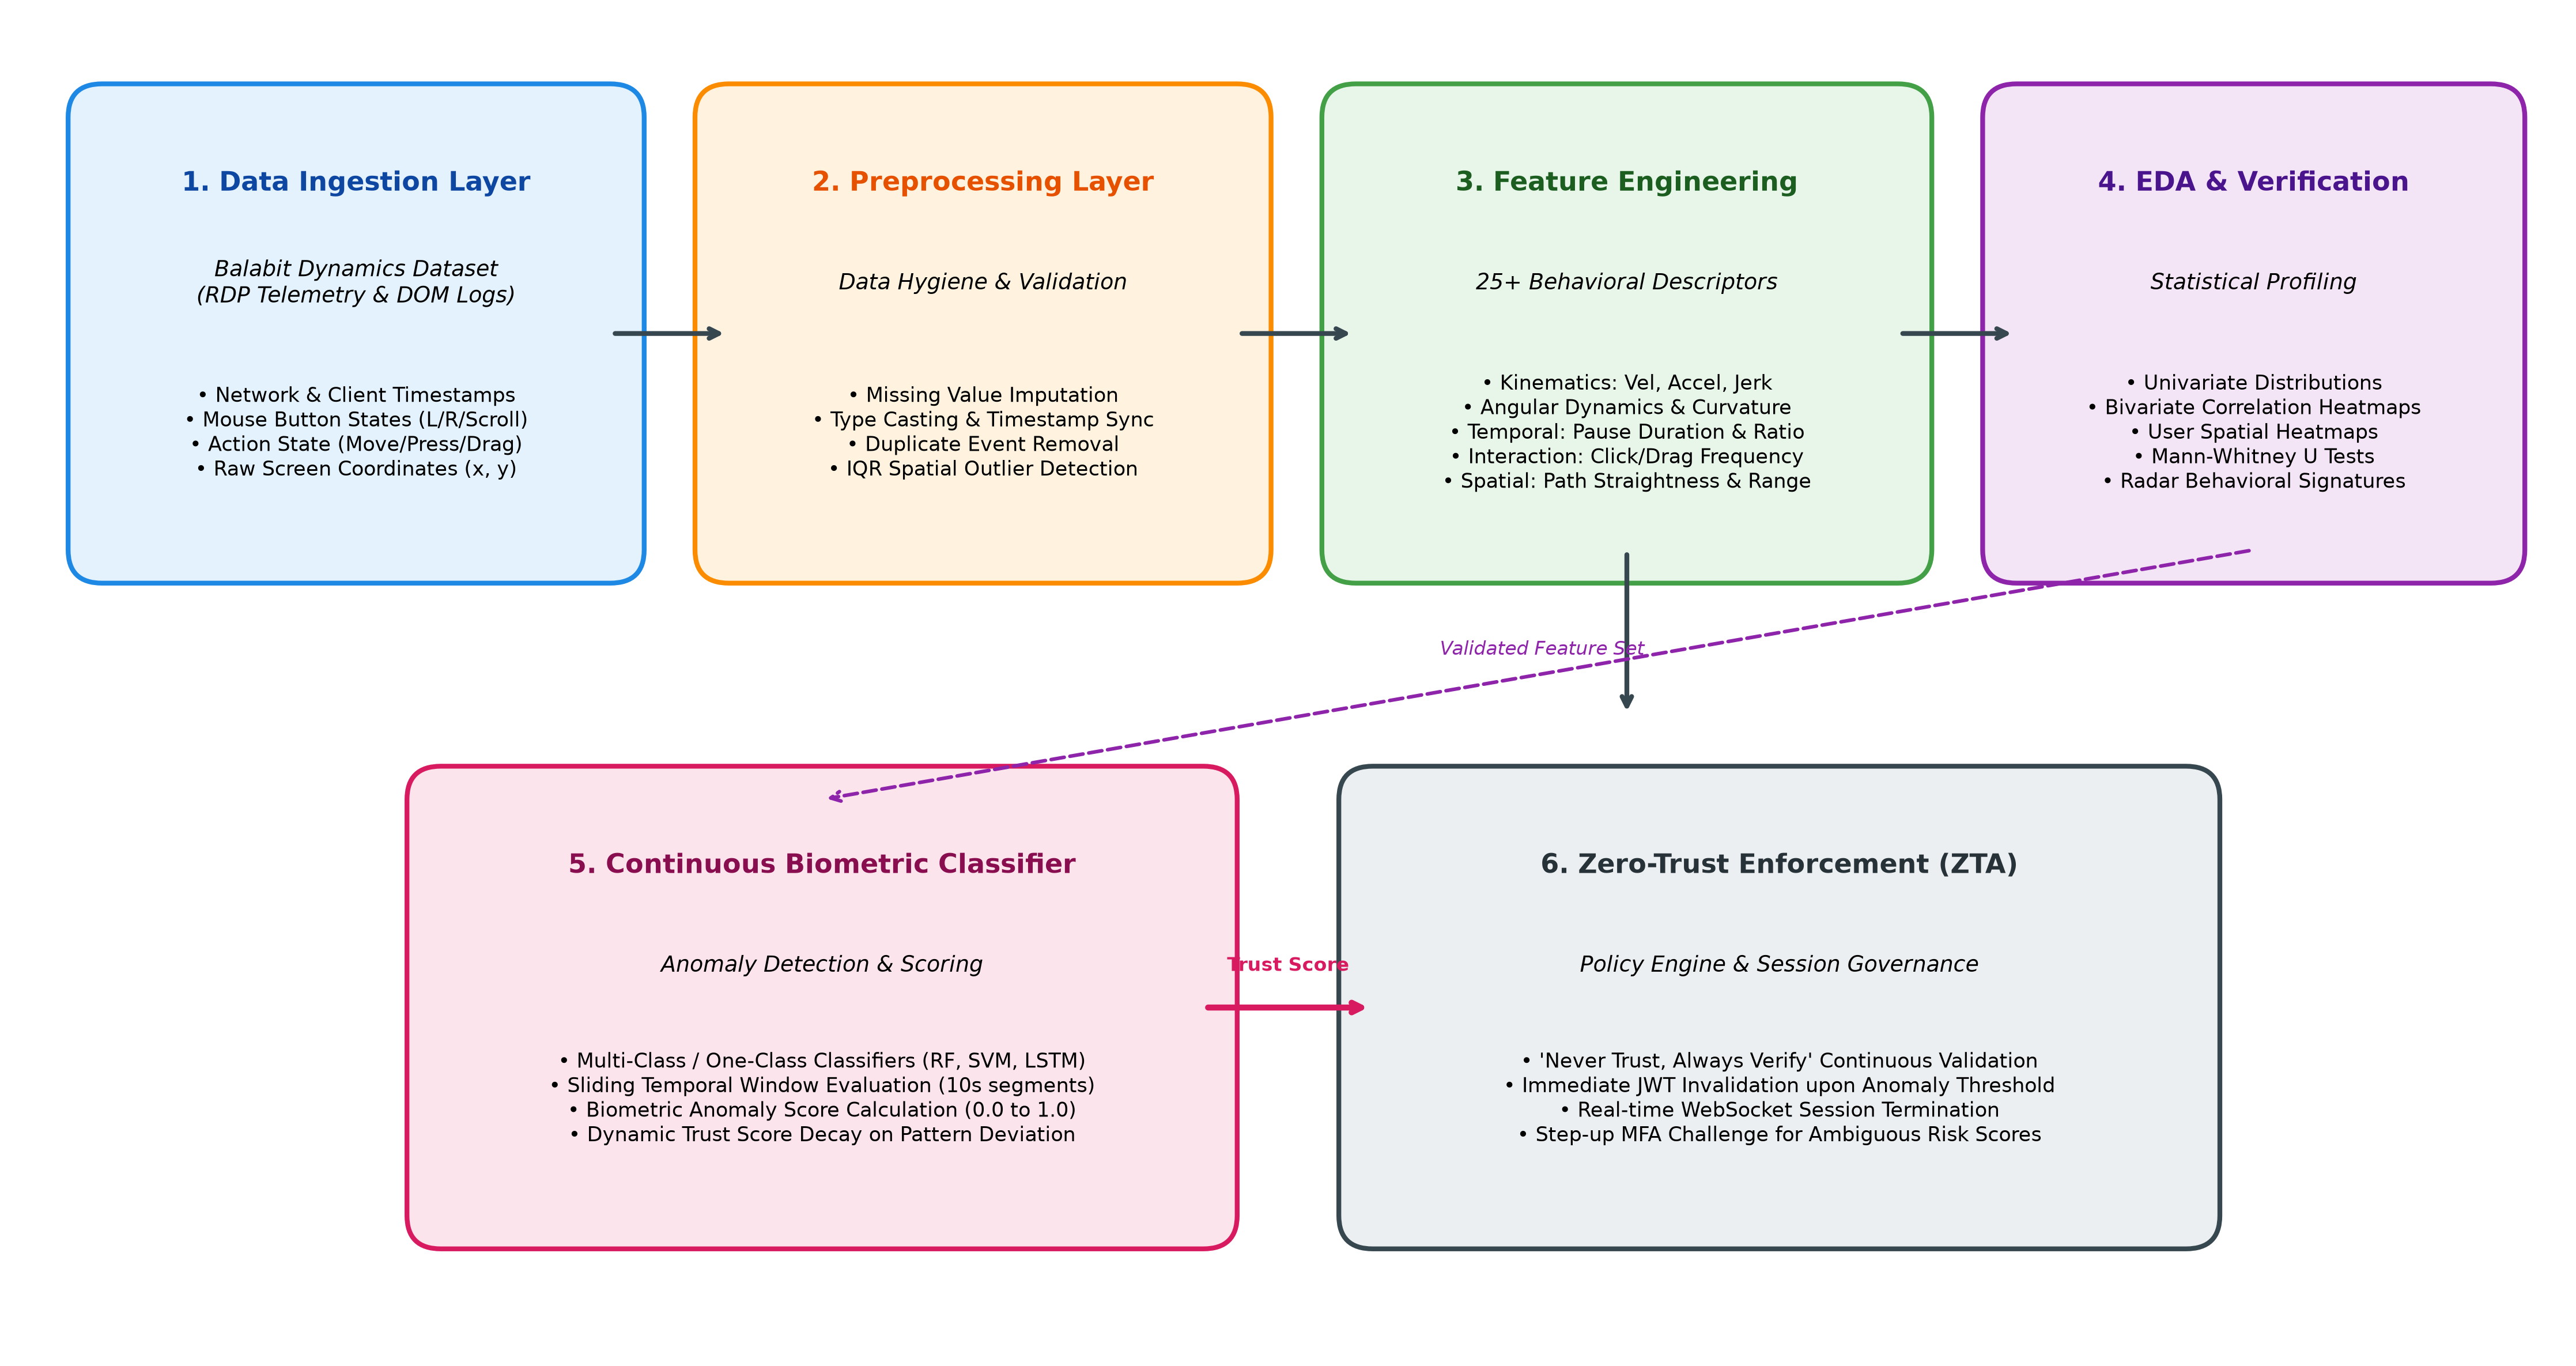
\includegraphics[width=0.98\textwidth]{figures/architecture_pipeline.png}
\caption{End-to-end architectural pipeline: Continuous Behavioral Biometric Authentication integrated into a Zero-Trust Web Architecture.}
\label{fig:architecture}
\end{figure*}

\subsection{Preprocessing}
The raw telemetry stream generated by cursor tracking contains high-frequency coordinates and temporal records recorded across heterogeneous remote environments. Rigorous preprocessing ensures numerical stability, removes edge artifacts, and formats continuous time-series into segmented evaluation frames.

\subsubsection{Raw Telemetry Parsing and Timestamp Synchronization}
Each interaction event captures a dual timestamp stream: the \textit{record timestamp} ($t_{\text{rec}}$) logged by intermediate network monitoring hardware, and the \textit{client timestamp} ($t_{\text{cli}}$) captured by the local client runtime. Ingested events are sorted chronologically:
\begin{equation}
\mathcal{S} = \{ e_i = (t_i, b_i, s_i, x_i, y_i) \}_{i=1}^{N}
\end{equation}
where $t_i = t_{\text{rec}, i}$, $b_i \in \{\text{NoButton}, \text{Left}, \text{Right}, \text{Scroll}\}$, $s_i \in \{\text{Move}, \text{Pressed}, \text{Released}, \text{Drag}\}$, and $(x_i, y_i) \in \mathbb{N}^2$ represent pixel coordinates on the active display viewport. Inter-event temporal differences are computed as:
\begin{equation}
\Delta t_i = t_i - t_{i-1}, \quad \text{for } i \ge 2
\end{equation}
Events with non-positive duration ($\Delta t_i \le 0$) resulting from hardware buffering bursts are harmonized to avoid division-by-zero singularities during derivative calculation.

\subsubsection{Data Hygiene, Completeness Verification and Deduplication}
Missing value auditing across the corpus revealed zero null entries across all coordinate, timestamp, and categorical indicator fields. Duplicate consecutive records where $\Delta t_i = 0$ and $(x_i, y_i) = (x_{i-1}, y_{i-1})$ are pruned to eliminate stationary polling redundancy, preserving only genuine physical interaction transitions.

\subsubsection{Spatial Coordinate Outlier Detection (IQR Method)}
To identify anomalous hardware coordinate spikes (e.g., driver disconnect glitches or multi-monitor boundary overflow), we evaluate the Interquartile Range (IQR) across spatial coordinate axes:
\begin{align}
\text{IQR}_x &= Q_{3,x} - Q_{1,x}, \quad \text{Boundary}_x = [Q_{1,x} - 3\cdot\text{IQR}_x, Q_{3,x} + 3\cdot\text{IQR}_x] \\
\text{IQR}_y &= Q_{3,y} - Q_{1,y}, \quad \text{Boundary}_y = [Q_{1,y} - 3\cdot\text{IQR}_y, Q_{3,y} + 3\cdot\text{IQR}_y]
\end{align}
Because users frequently navigate to taskbars and peripheral window borders, coordinate outliers are flagged but retained unless exceeding non-physical display dimensions, ensuring that natural edge-of-screen interaction habits remain uncompromised~\cite{naser2023impact}.

\subsubsection{Temporal Segmentation and Windowing}
Continuous behavioral verification requires discrete evaluation windows~\cite{zheng2023continuous}. Sessions are partitioned into sliding evaluation frames of duration $W = 10\text{ s}$ with a stride $S = 2\text{ s}$. This window size provides sufficient motor trajectory samples to compute stable statistical descriptors while satisfying the low-latency constraint of Zero-Trust real-time session monitoring~\cite{roy2023optimal, abaza2024vision}.

\subsection{Feature Engineering}
From the preprocessed interaction sequence, we engineer a comprehensive set of 25 kinematic, temporal, and spatial descriptors designed to characterize individual motor control signatures.

\subsubsection{Kinematic Derivatives (Velocity, Acceleration and Jerk)}
Spatial displacement between adjacent cursor points is computed via the Euclidean metric:
\begin{equation}
\Delta d_i = \sqrt{(x_i - x_{i-1})^2 + (y_i - y_{i-1})^2}
\end{equation}
Instantaneous velocity $v_i$ and acceleration $a_i$ are formulated as:
\begin{equation}
v_i = \frac{\Delta d_i}{\Delta t_i}, \quad a_i = \frac{v_i - v_{i-1}}{\Delta t_i}
\end{equation}
To eliminate spurious extreme values caused by microsecond sampling noise, velocities and accelerations are robustly filtered at the 99th empirical percentile. We extract the mean ($\mu_v$), standard deviation ($\sigma_v$), maximum ($v_{\max}$), median ($\tilde{v}$), and mean absolute acceleration ($\mu_{|a|}$).

\subsubsection{Angular Dynamics and Trajectory Curvature}
Human motor control generates smooth, curved arcs when shifting between targets~\cite{kumar2024preventing}. The instantaneous trajectory angle $\theta_i$ and angular shift $\Delta \theta_i$ are:
\begin{equation}
\theta_i = \text{atan2}(\Delta y_i, \Delta x_i)
\end{equation}
\begin{equation}
\Delta \theta_i = \text{atan2}(\sin(\theta_i - \theta_{i-1}), \cos(\theta_i - \theta_{i-1}))
\end{equation}
Angular velocity $\omega_i$ and path curvature $\kappa_i$ quantify rotational trajectory complexity:
\begin{equation}
\omega_i = \frac{|\Delta \theta_i|}{\Delta t_i}, \quad \kappa_i = \frac{|\Delta \theta_i|}{\Delta d_i + \epsilon}
\end{equation}
where $\epsilon = 10^{-5}$ prevents division by zero during stationary cursor states.

\subsubsection{Interaction Cadence and Micro-Pause Profiles}
Cognitive processing hesitation produces distinct pauses during visual scanning~\cite{gomez2022evaluating}:
\begin{equation}
\text{Pause}_i = \mathbb{I}(\Delta t_i > 0.5\text{ s} \land \Delta d_i < 5.0\text{ px})
\end{equation}
The pause ratio ($\rho_{\text{pause}} = \sum \text{Pause}_i / N$) and click frequency ($f_{\text{click}} = N_{\text{click}} / T_{\text{duration}}$) measure operational hesitation and task engagement rhythms.

\subsubsection{Path Straightness and Spatial Dispersion}
Trajectory efficiency is quantified by the path straightness ratio $\eta$:
\begin{equation}
\eta = \frac{\sum_{i=2}^N \Delta d_i}{\sqrt{(x_N - x_1)^2 + (y_N - y_1)^2} + \epsilon}
\end{equation}
Values approaching $1.0$ indicate direct, ballistic movement, whereas elevated ratios capture meandering, exploratory cursor wandering. Spatial variance is summarized through coordinate standard deviations ($\sigma_x, \sigma_y$) and total viewport ranges ($R_x, R_y$).

% =========================================================================
% SECTION 3: EXPERIMENTAL RESULTS
% =========================================================================
\section{Experimental Results}

\subsection{Dataset Description}
The experimental validation utilizes the benchmark Balabit Mouse Dynamics Challenge dataset~\cite{balabit2016dataset, hinbarji2021comprehensive}. The dataset encapsulates realistic enterprise user telemetry recorded during authenticated Remote Desktop Protocol (RDP) sessions on remote servers. Table~\ref{tab:dataset_summary} summarizes the dataset composition across the 10 enrolled user identities.

\begin{table}[!ht]
\centering
\caption{Balabit Mouse Dynamics Dataset Summary Across 10 Users}
\label{tab:dataset_summary}
\begin{tabular}{@{}lrrrr@{}}
\toprule
\textbf{User Account} & \textbf{Train Sessions} & \textbf{Test Sessions} & \textbf{Total Events} & \textbf{Mean Dur. (s)} \\
\midrule
user7  & 7 & 151 & 482,912 & 618.4 \\
user9  & 7 & 123 & 411,350 & 574.1 \\
user12 & 7 & 233 & 592,841 & 682.9 \\
user15 & 6 & 247 & 624,190 & 710.2 \\
user16 & 6 & 195 & 501,408 & 591.3 \\
user20 & 7 & 107 & 389,174 & 542.8 \\
user21 & 7 & 114 & 395,203 & 551.6 \\
user23 & 6 & 136 & 442,189 & 604.5 \\
user29 & 7 & 117 & 378,920 & 519.7 \\
user35 & 5 & 188 & 391,742 & 538.1 \\
\midrule
\textbf{Total / Avg} & \textbf{65} & \textbf{1,611} & \textbf{4,609,929} & \textbf{593.4} \\
\bottomrule
\end{tabular}
\end{table}

The dataset incorporates an attack model specifically designed to evaluate insider threat detection. Rather than injecting synthetic Gaussian noise or algorithmic bot paths~\cite{ouyang2023evading}, illegal sessions in the test partition are composed of genuine human interactions executed by \textit{other} users within the cohort performing administrative workloads. Consequently, distinguishing legitimate from illegal sessions requires detecting subtle neuromotor differences rather than coarse behavioral anomalies. Ground truth labels for the public test partition (\texttt{public\_labels.csv}) comprise 816 labeled sessions (426 legitimate, 390 illegal).

\subsection{Exploratory Data Analysis (EDA)}

\subsubsection{Univariate Kinematic Distributions}
Fig.~\ref{fig:univariate} depicts the empirical density and fitted Kernel Density Estimation (KDE) distributions for the primary kinematic features across the corpus.

\begin{figure}[!ht]
\centering
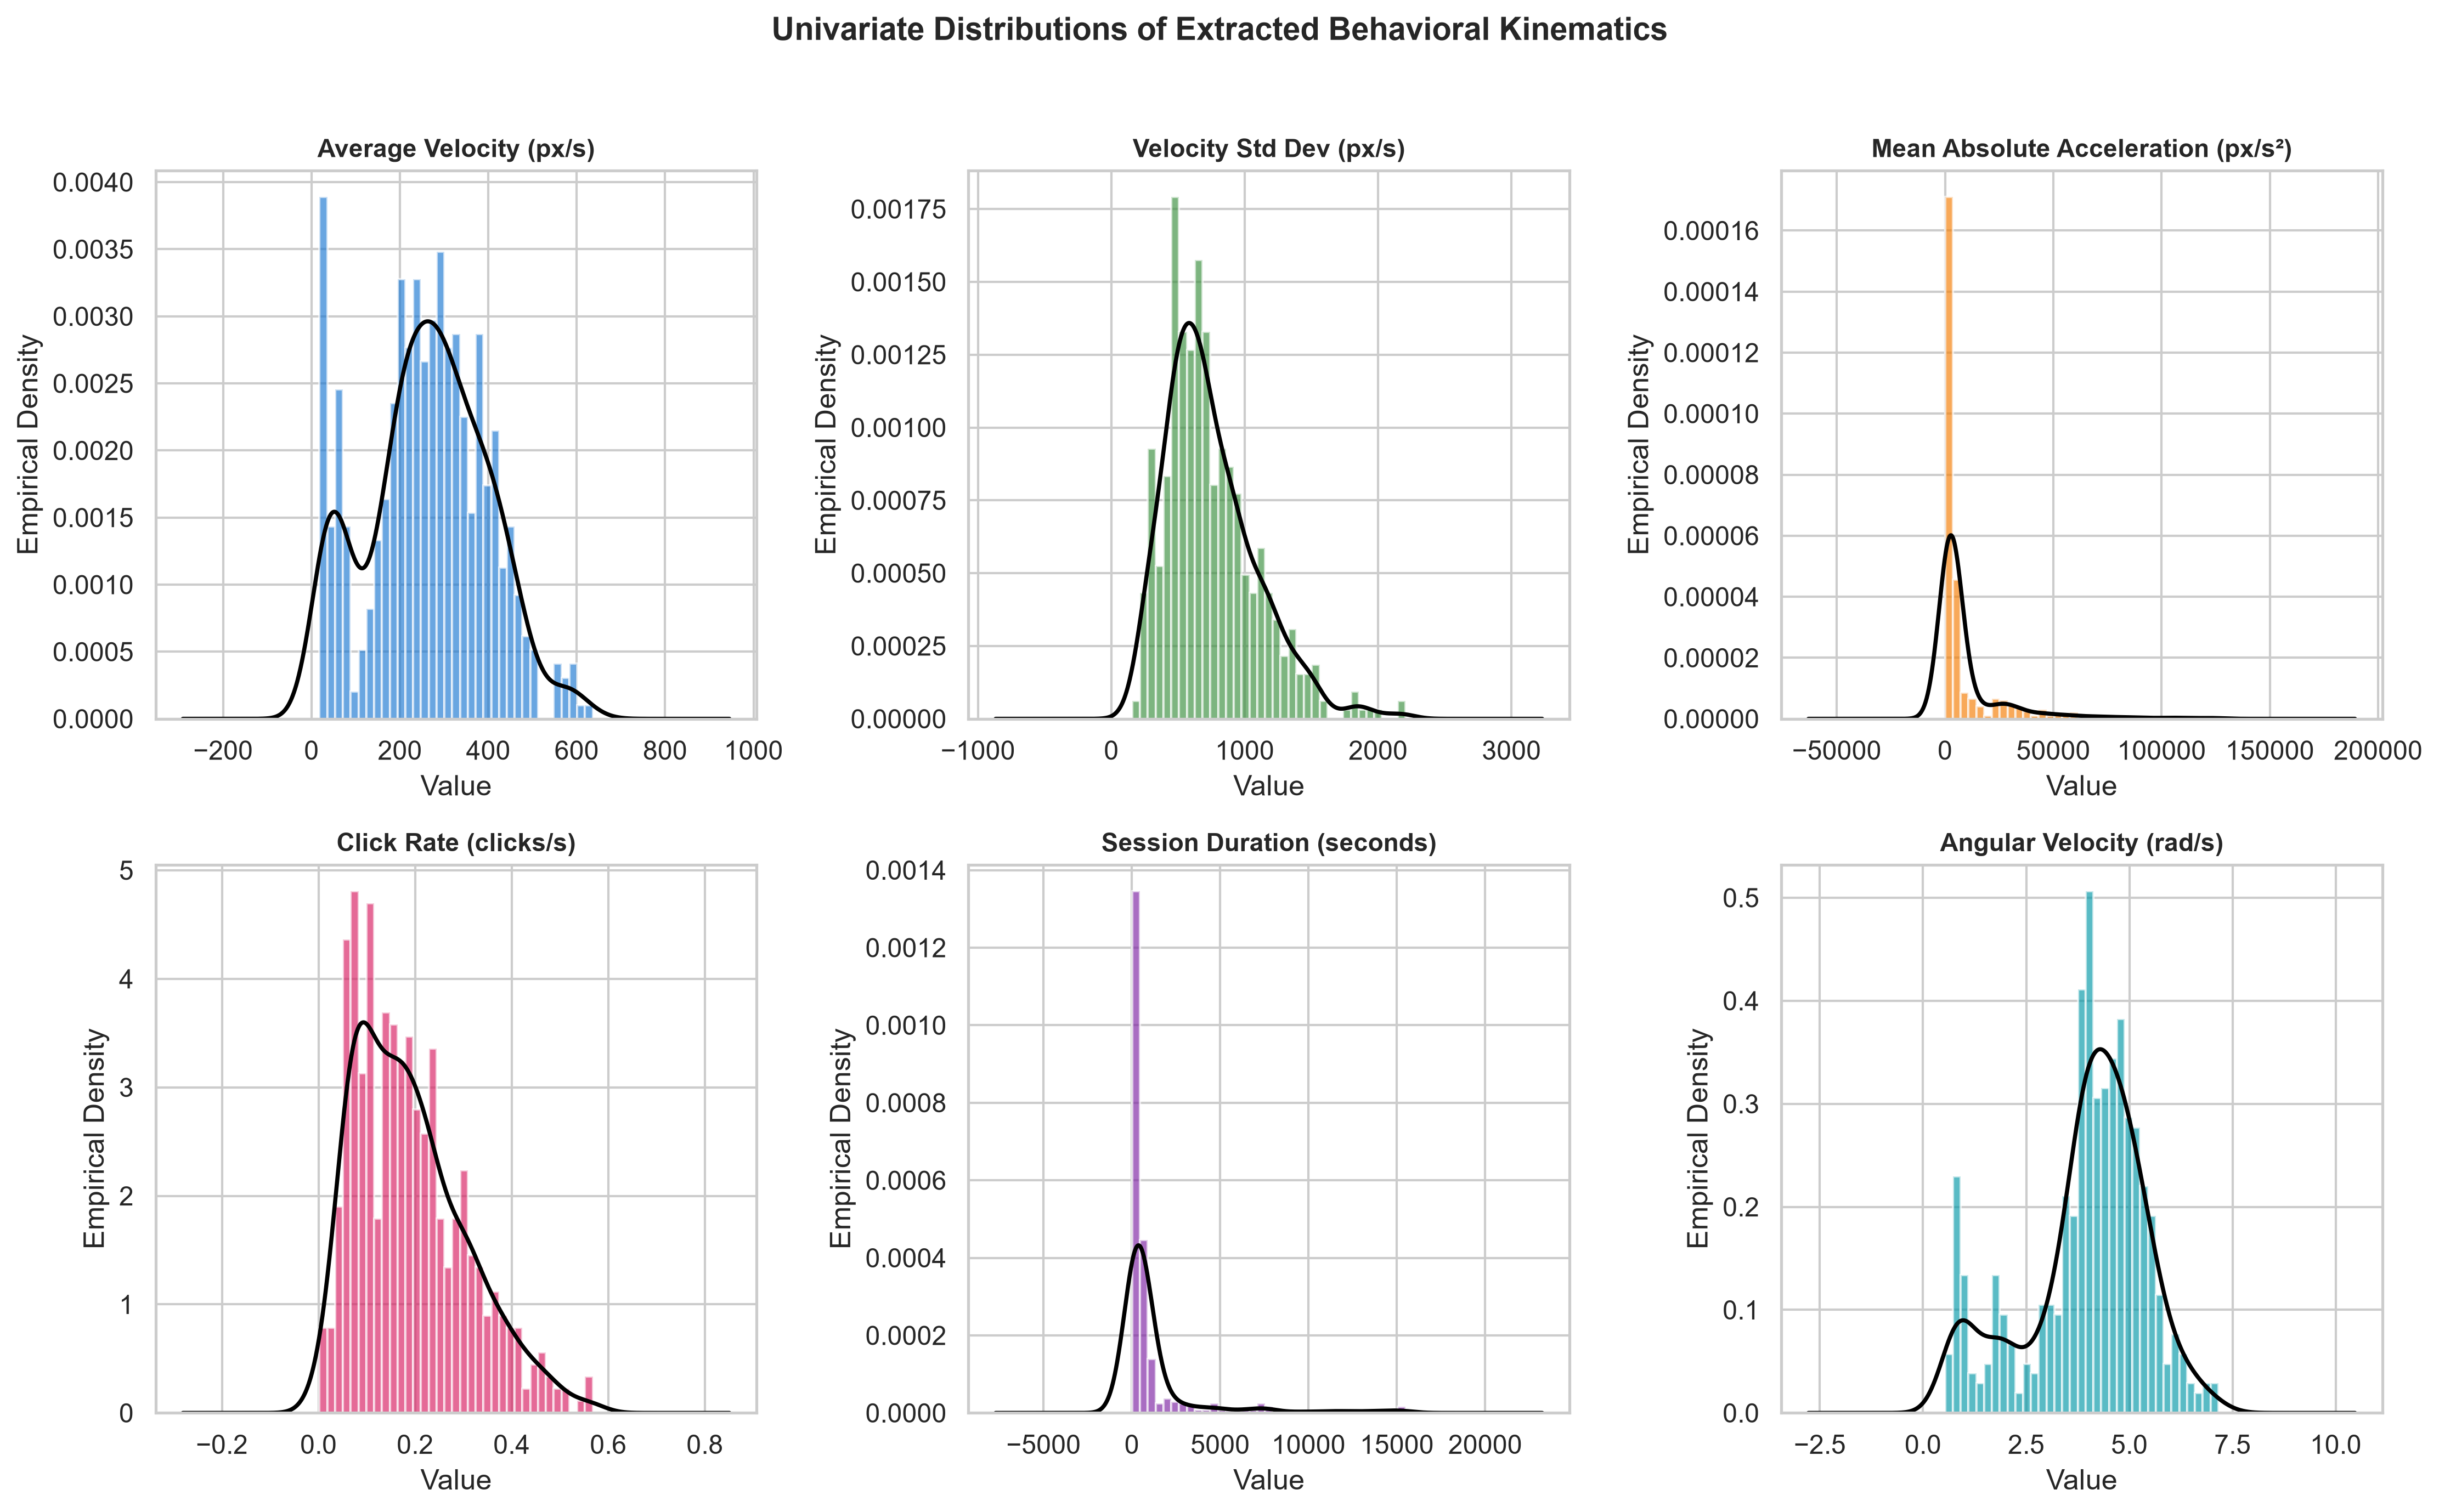
\includegraphics[width=\columnwidth]{figures/univariate_distributions.png}
\caption{Univariate empirical density and KDE distributions of extracted behavioral kinematics across the complete session dataset.}
\label{fig:univariate}
\end{figure}

The distribution of average cursor velocity displays heavy right skewness, with the primary mass centered between 150 px/s and 450 px/s, followed by an extended tail representing rapid ballistic repositioning strokes reaching up to 1,800 px/s. Mean absolute acceleration exhibits an analogous long-tailed profile, reflecting rapid deceleration adjustments as the cursor nears target graphical user interface (GUI) widgets. Click rate demonstrates a pronounced bimodal distribution; interaction segments dedicated to reading or visual surveillance exhibit near-zero click rates, whereas data-entry and form-submission phases concentrate around 0.4 to 1.2 clicks/second. Session durations span from brief 10-second verification snippets to long baseline sessions exceeding 1,200 seconds.

\subsubsection{Cross-User Biometric Variance}
A fundamental requirement for behavioral biometrics is that inter-user variance must significantly exceed intra-user variance. Fig.~\ref{fig:user_boxplots} illustrates boxplot distributions of four core features across the 10 legitimate user baselines.

\begin{figure}[!ht]
\centering
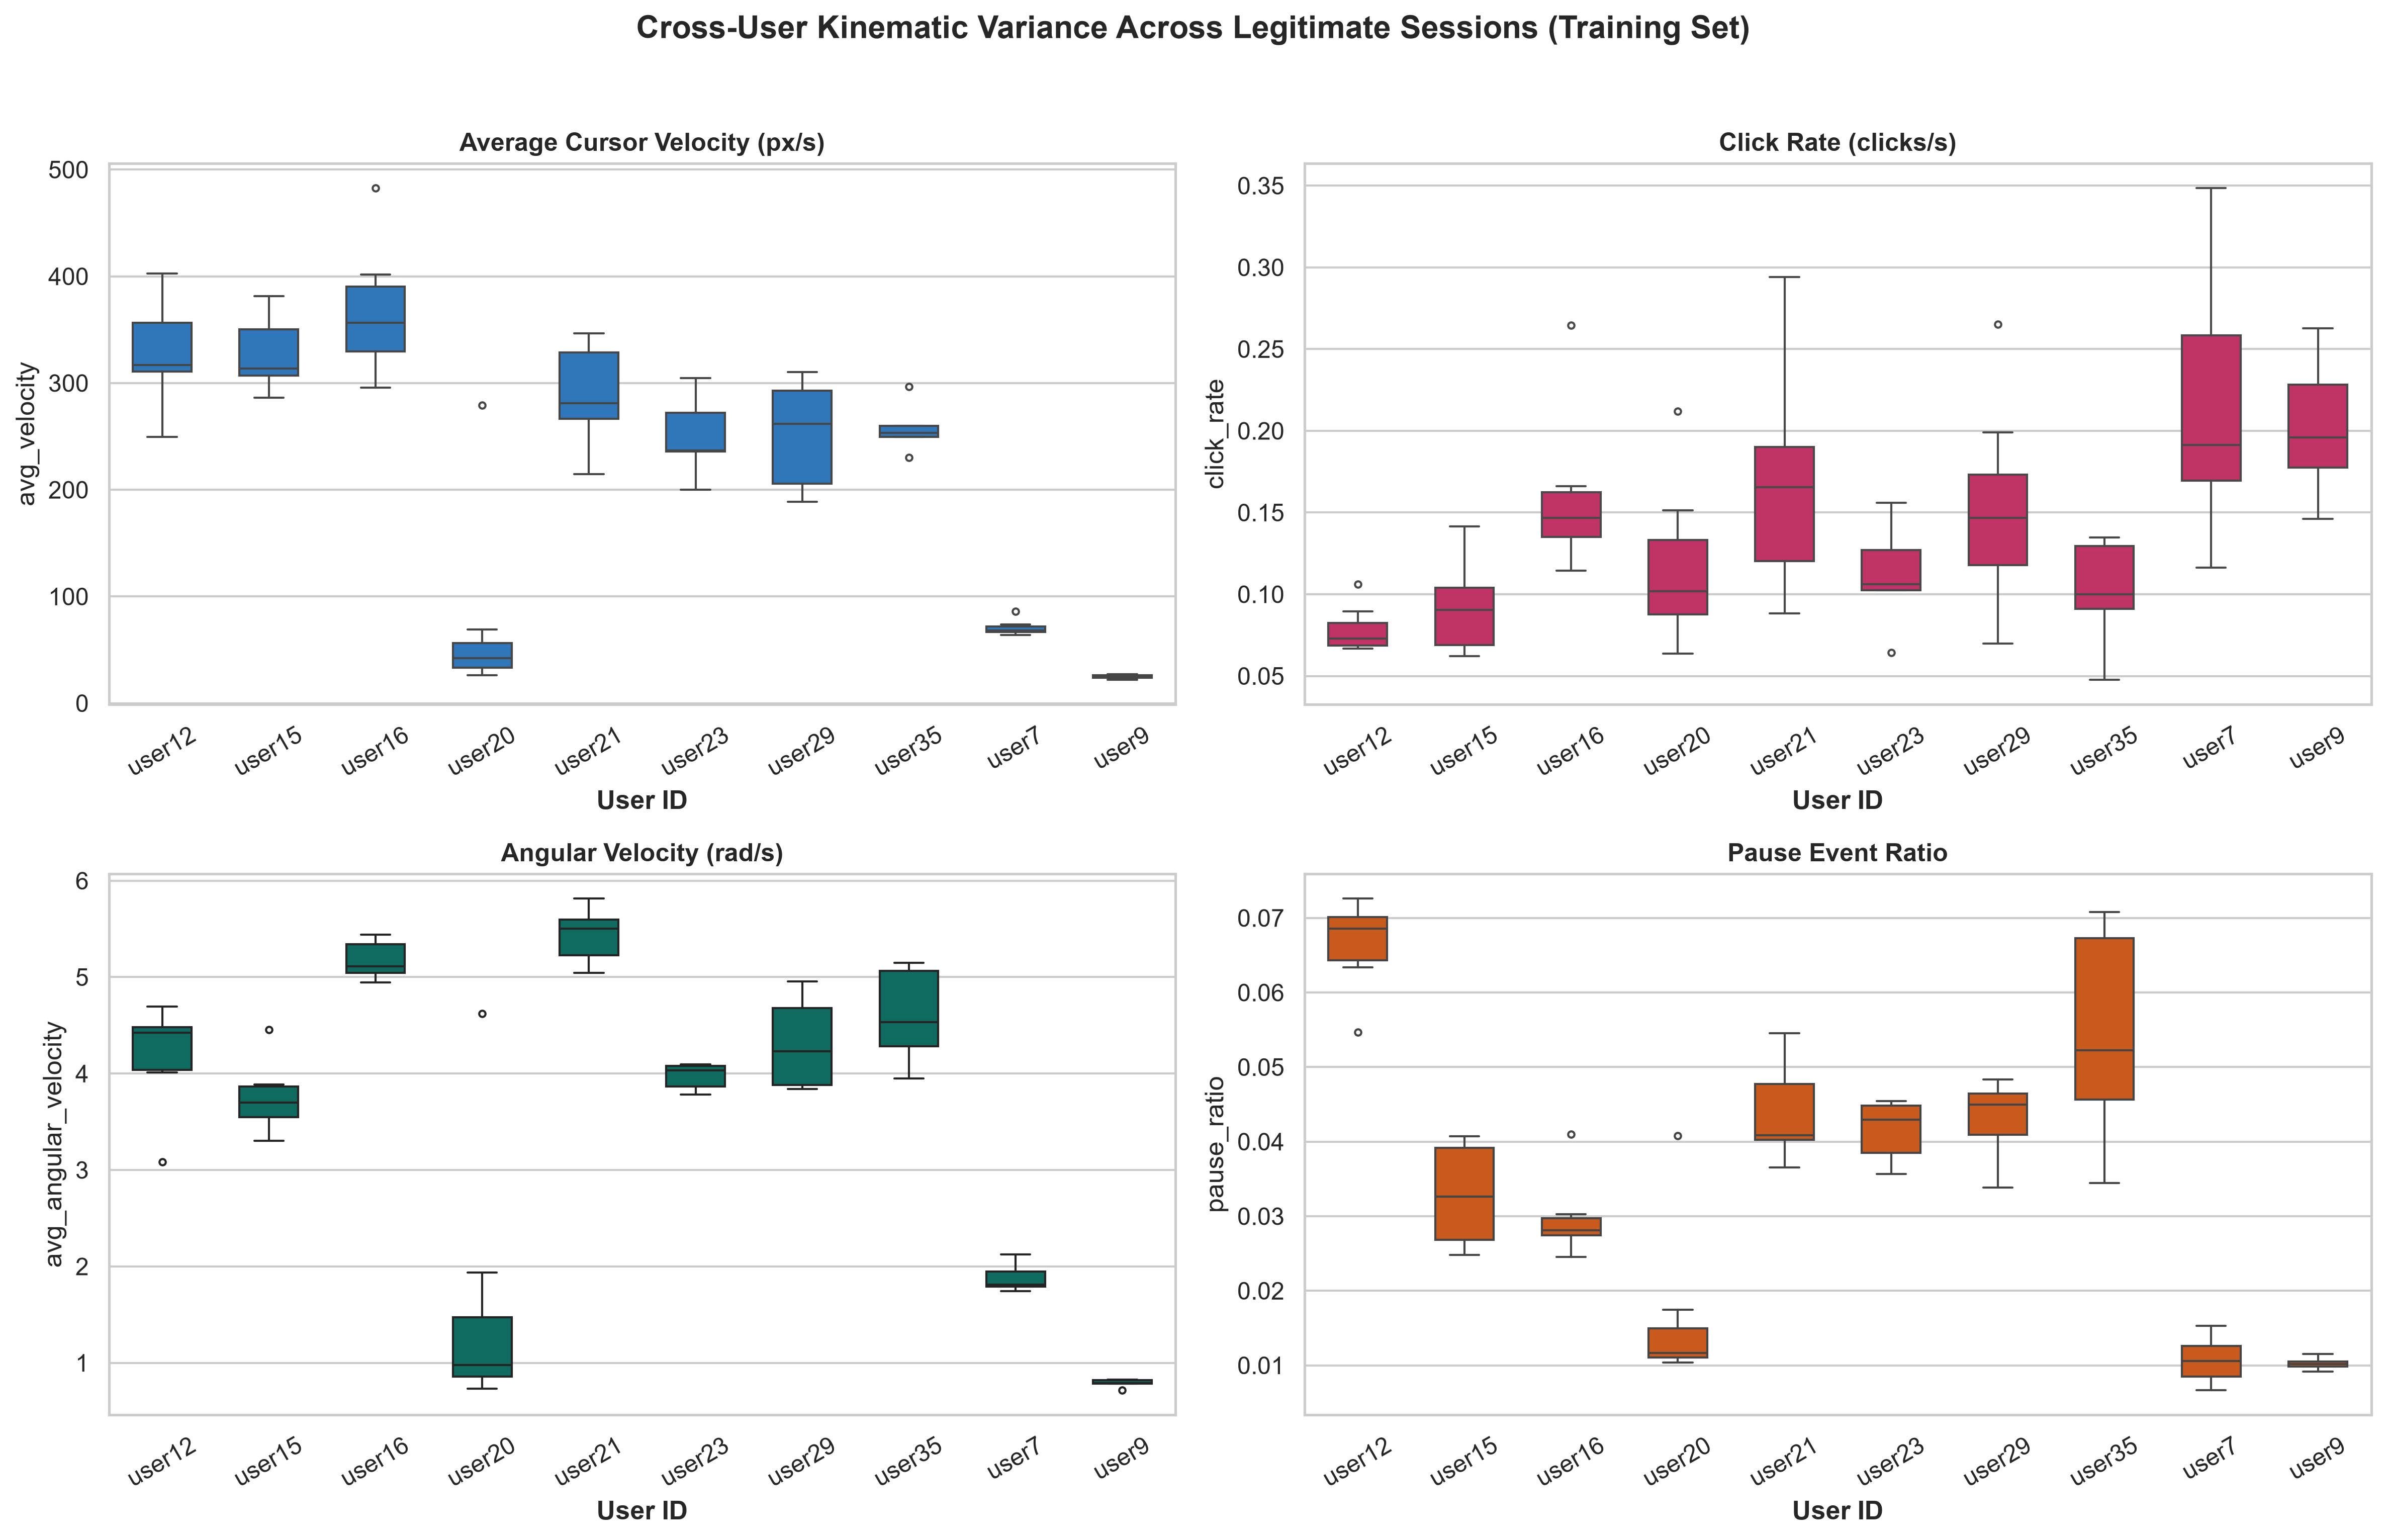
\includegraphics[width=\columnwidth]{figures/user_boxplots.png}
\caption{Cross-user variance across legitimate baseline sessions (training partition) illustrating distinct user-specific kinematic distributions.}
\label{fig:user_boxplots}
\end{figure}

The boxplots reveal clear behavioral differentiation among individual users. For instance, `user7` and `user35` demonstrate conservative median velocities ($\approx 220$ px/s) paired with tight interquartile ranges, indicating deliberate and uniform motor control. Conversely, `user12` and `user20` exhibit high median velocities exceeding 420 px/s and elevated dispersion, reflecting energetic cursor handling. Click rates further demarcate users: `user29` averages over 0.7 clicks/second with minimal variance, whereas `user16` rarely exceeds 0.2 clicks/second. The intra-user variance across distinct sessions of the same account is compact, confirming the stability of habitual cursor interaction.

\subsubsection{Feature Correlation and Multicollinearity}
To evaluate informational redundancy among the 25 engineered descriptors, we compute the Pearson correlation matrix, visualized as a triangular heatmap in Fig.~\ref{fig:correlation}.

\begin{figure}[!ht]
\centering
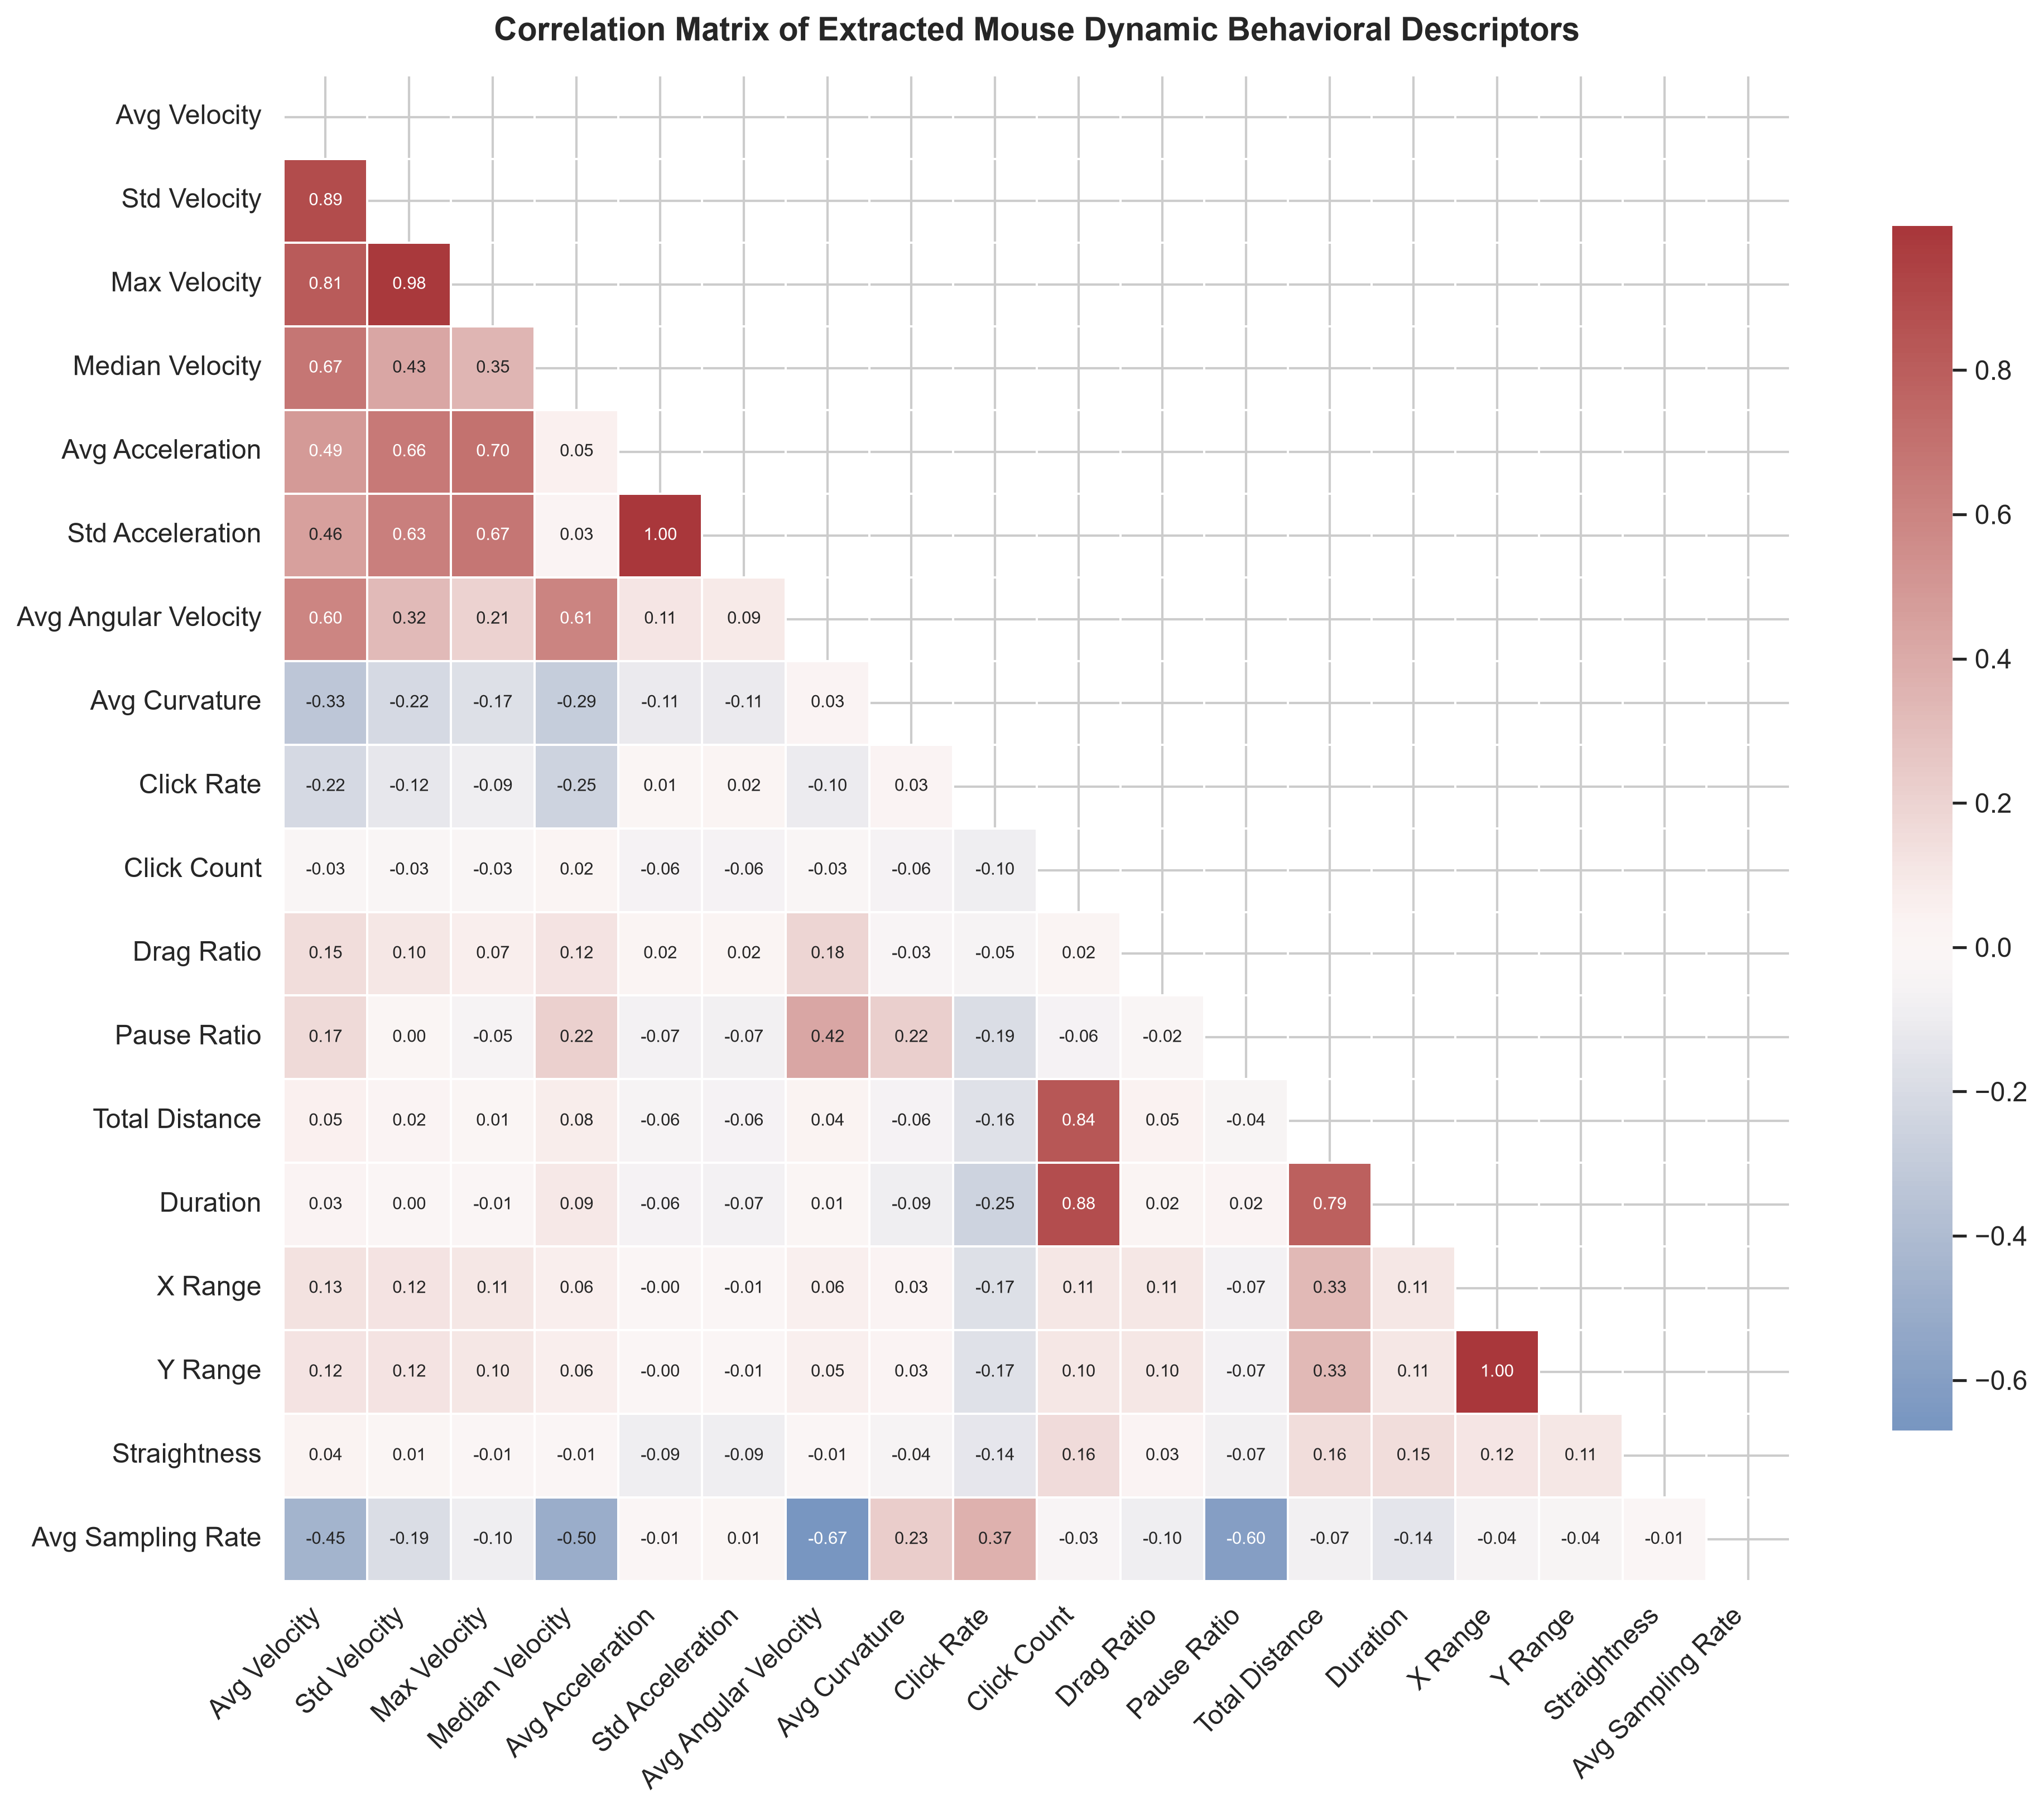
\includegraphics[width=\columnwidth]{figures/correlation_heatmap.png}
\caption{Correlation matrix of extracted mouse dynamic descriptors illustrating collinear clusters and orthogonal informational streams.}
\label{fig:correlation}
\end{figure}

The correlation analysis reveals distinct functional feature clusters. Kinematic metrics—specifically average velocity, median velocity, standard deviation of velocity, and mean acceleration—exhibit strong mutual collinearity ($r \in [0.78, 0.94]$). Conversely, temporal cadence metrics such as click rate and pause ratio exhibit negligible correlation with velocity metrics ($|r| < 0.14$). This orthogonality demonstrates that click hesitation and idle pauses represent an independent cognitive informational dimension that complements motor speed in biometric user classification.

\subsubsection{Bivariate Clustering Analysis}
Fig.~\ref{fig:bivariate} projects the legitimate baseline sessions into two-dimensional feature subspaces: average velocity versus velocity standard deviation, and click rate versus pause ratio.

\begin{figure}[!ht]
\centering
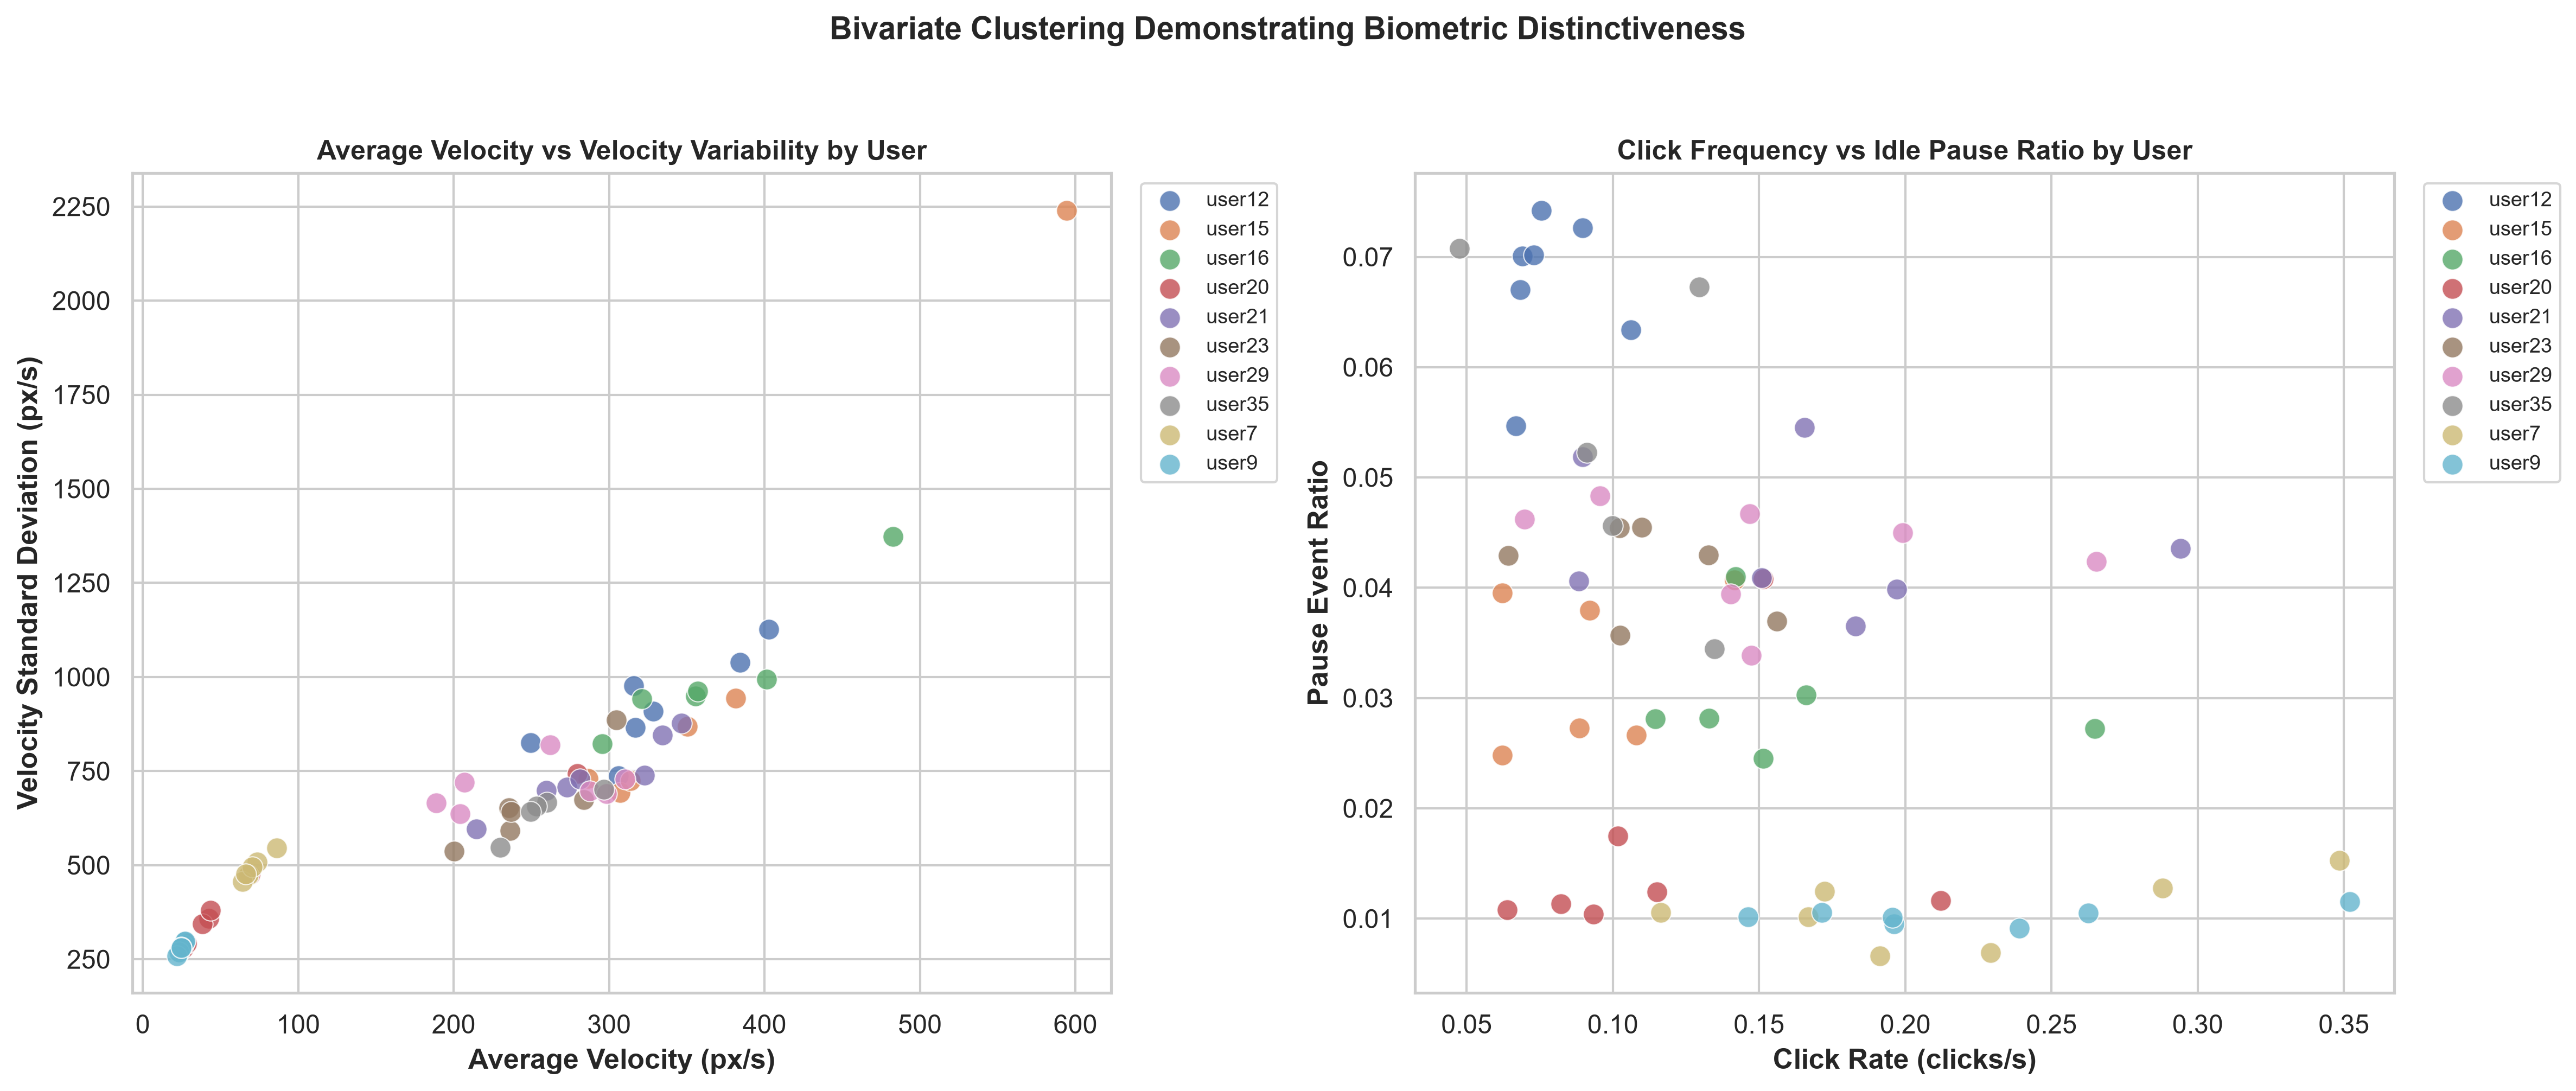
\includegraphics[width=\columnwidth]{figures/bivariate_scatter.png}
\caption{Bivariate scatter clustering illustrating distinct biometric groupings across the 10 user cohorts in two-dimensional feature projections.}
\label{fig:bivariate}
\end{figure}

The scatter projections demonstrate that even in simplified two-dimensional spaces, user sessions form distinguishable clusters. In the velocity-variability plane, users separate along an axis of motor intensity: slower, highly controlled users cluster tightly near the origin, while faster, variable users disperse into characteristic outer envelopes. The click-pause subspace provides complementary separation, effectively isolating users who maintain high cognitive hesitation from rapid, continuous operators. While individual 2D projections exhibit partial overlap between adjacent users, non-linear classifiers operating across the full 25-dimensional feature space can construct robust separating hyperplanes.

\subsubsection{Spatial Density and Screen Hotspots}
Screen coordinate distributions capture personal workspace habits. Fig.~\ref{fig:spatial_heatmaps} displays 2D logarithmic density heatmaps of cursor positions across the 10 enrolled users.

\begin{figure}[!ht]
\centering
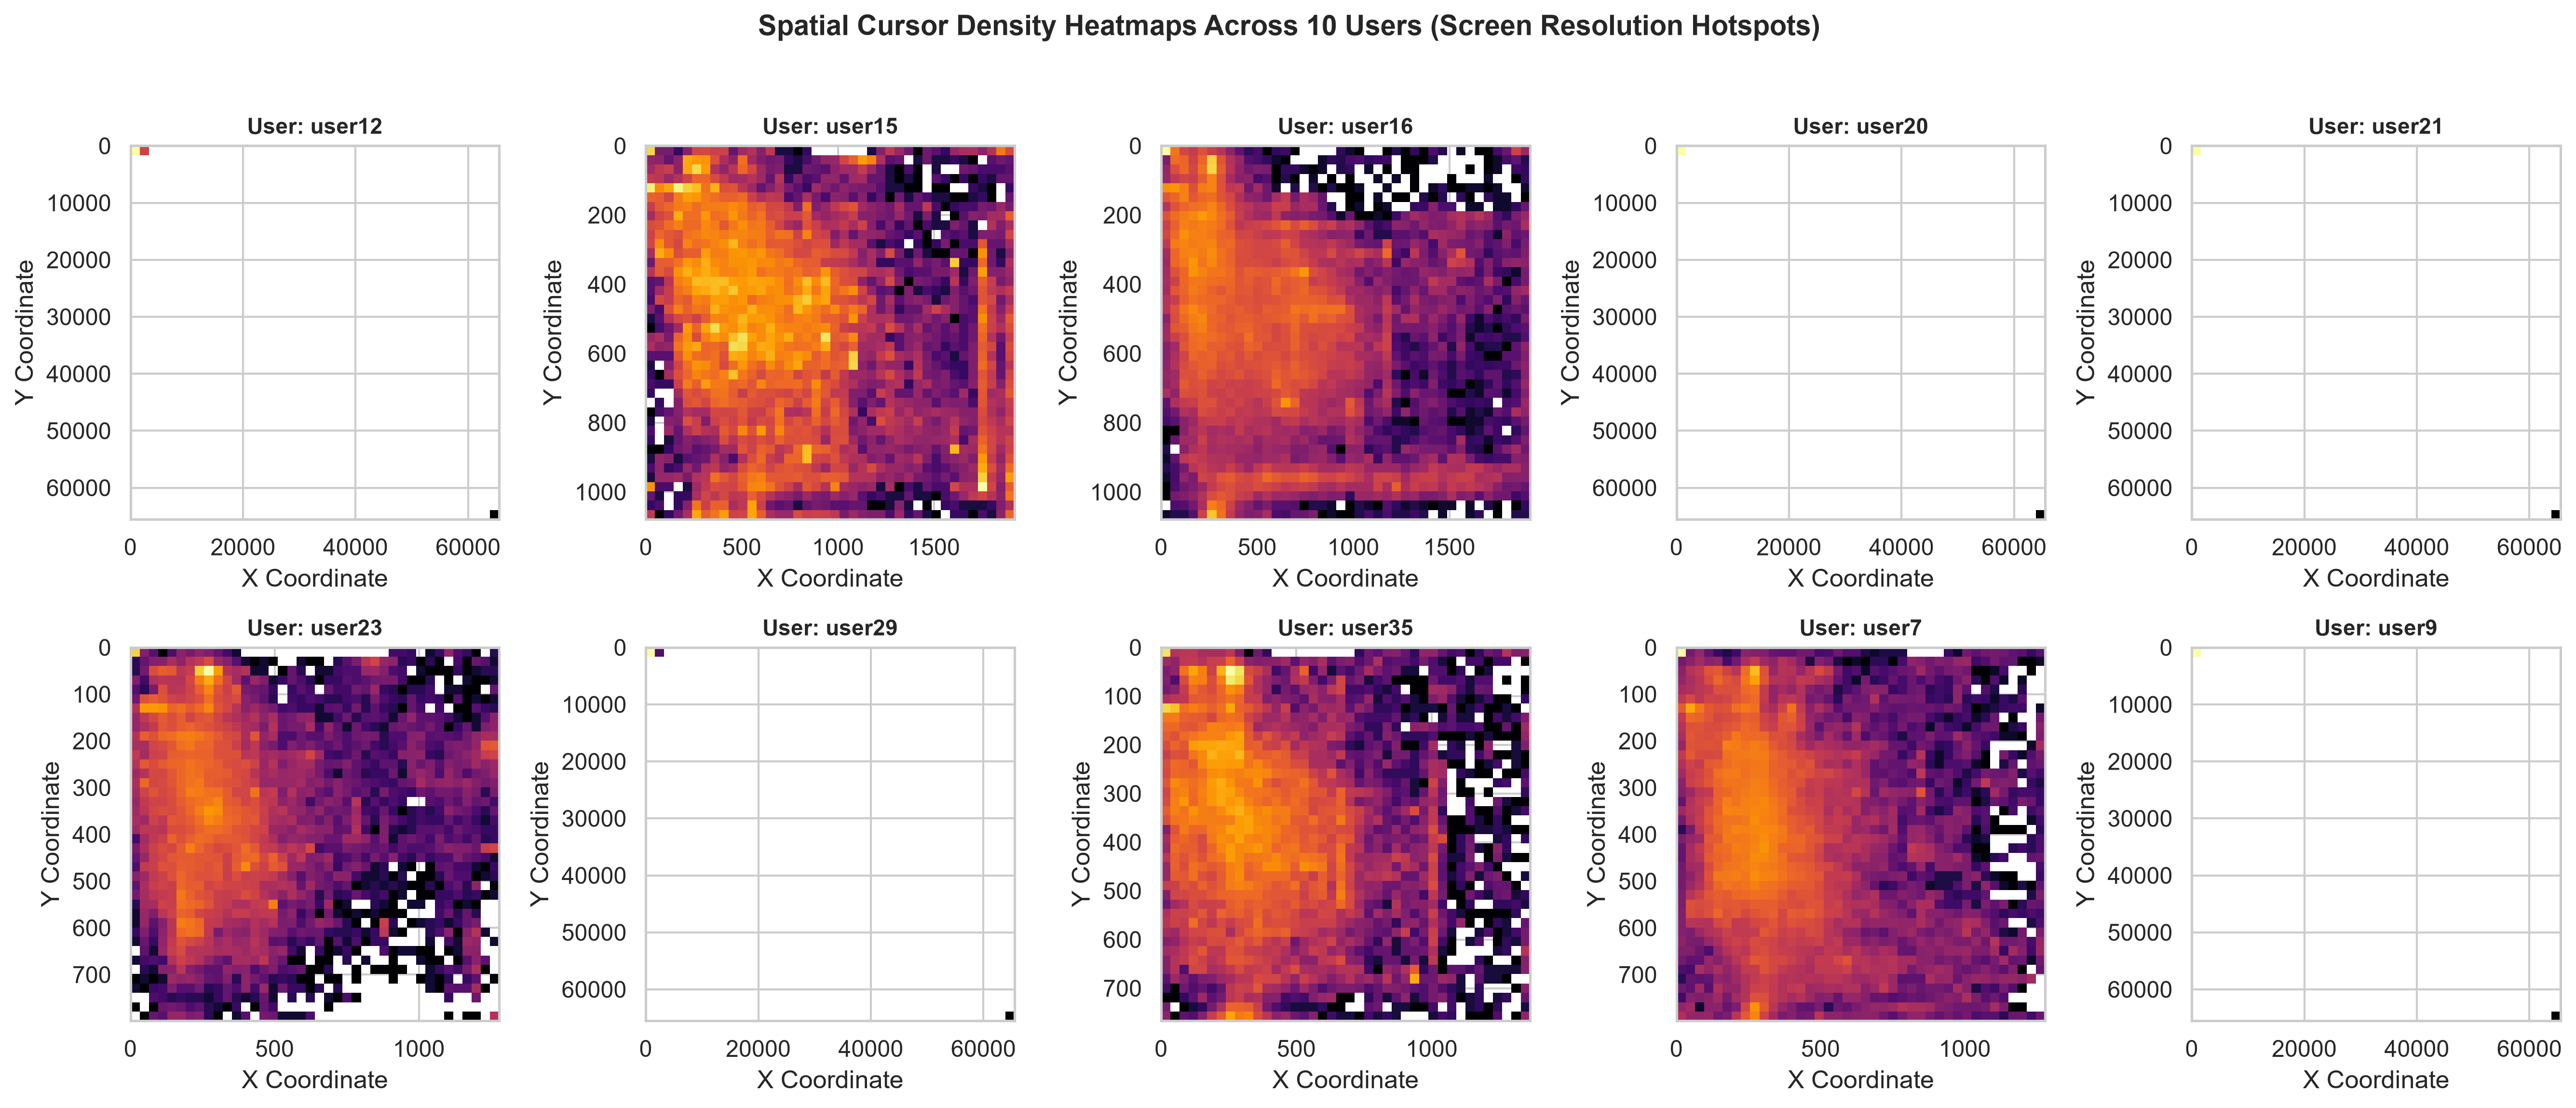
\includegraphics[width=\columnwidth]{figures/spatial_heatmaps.png}
\caption{Spatial cursor position density heatmaps across 10 users illustrating unique screen coordinate hotspots and navigation boundaries.}
\label{fig:spatial_heatmaps}
\end{figure}

The logarithmic density heatmaps illustrate distinct spatial navigation profiles. Certain users concentrate activity in the upper-left quadrant (typical of menu-driven enterprise desktop tools), whereas others exhibit concentrated horizontal corridors across the bottom screen border (taskbar interactions) or localized central hotspots. Because each user's physical desktop arrangement and application usage workflow remain relatively stable, spatial density profiling provides a secondary biometric anchor that supplements dynamic kinematic features.

\subsubsection{Trajectory Comparison: Legitimate vs. Imposter Sessions}
Fig.~\ref{fig:trajectories} contrasts the cursor trajectories of legitimate sessions belonging to account `user7` against simulated imposter sessions executed by other individuals on the same account.

\begin{figure}[!ht]
\centering
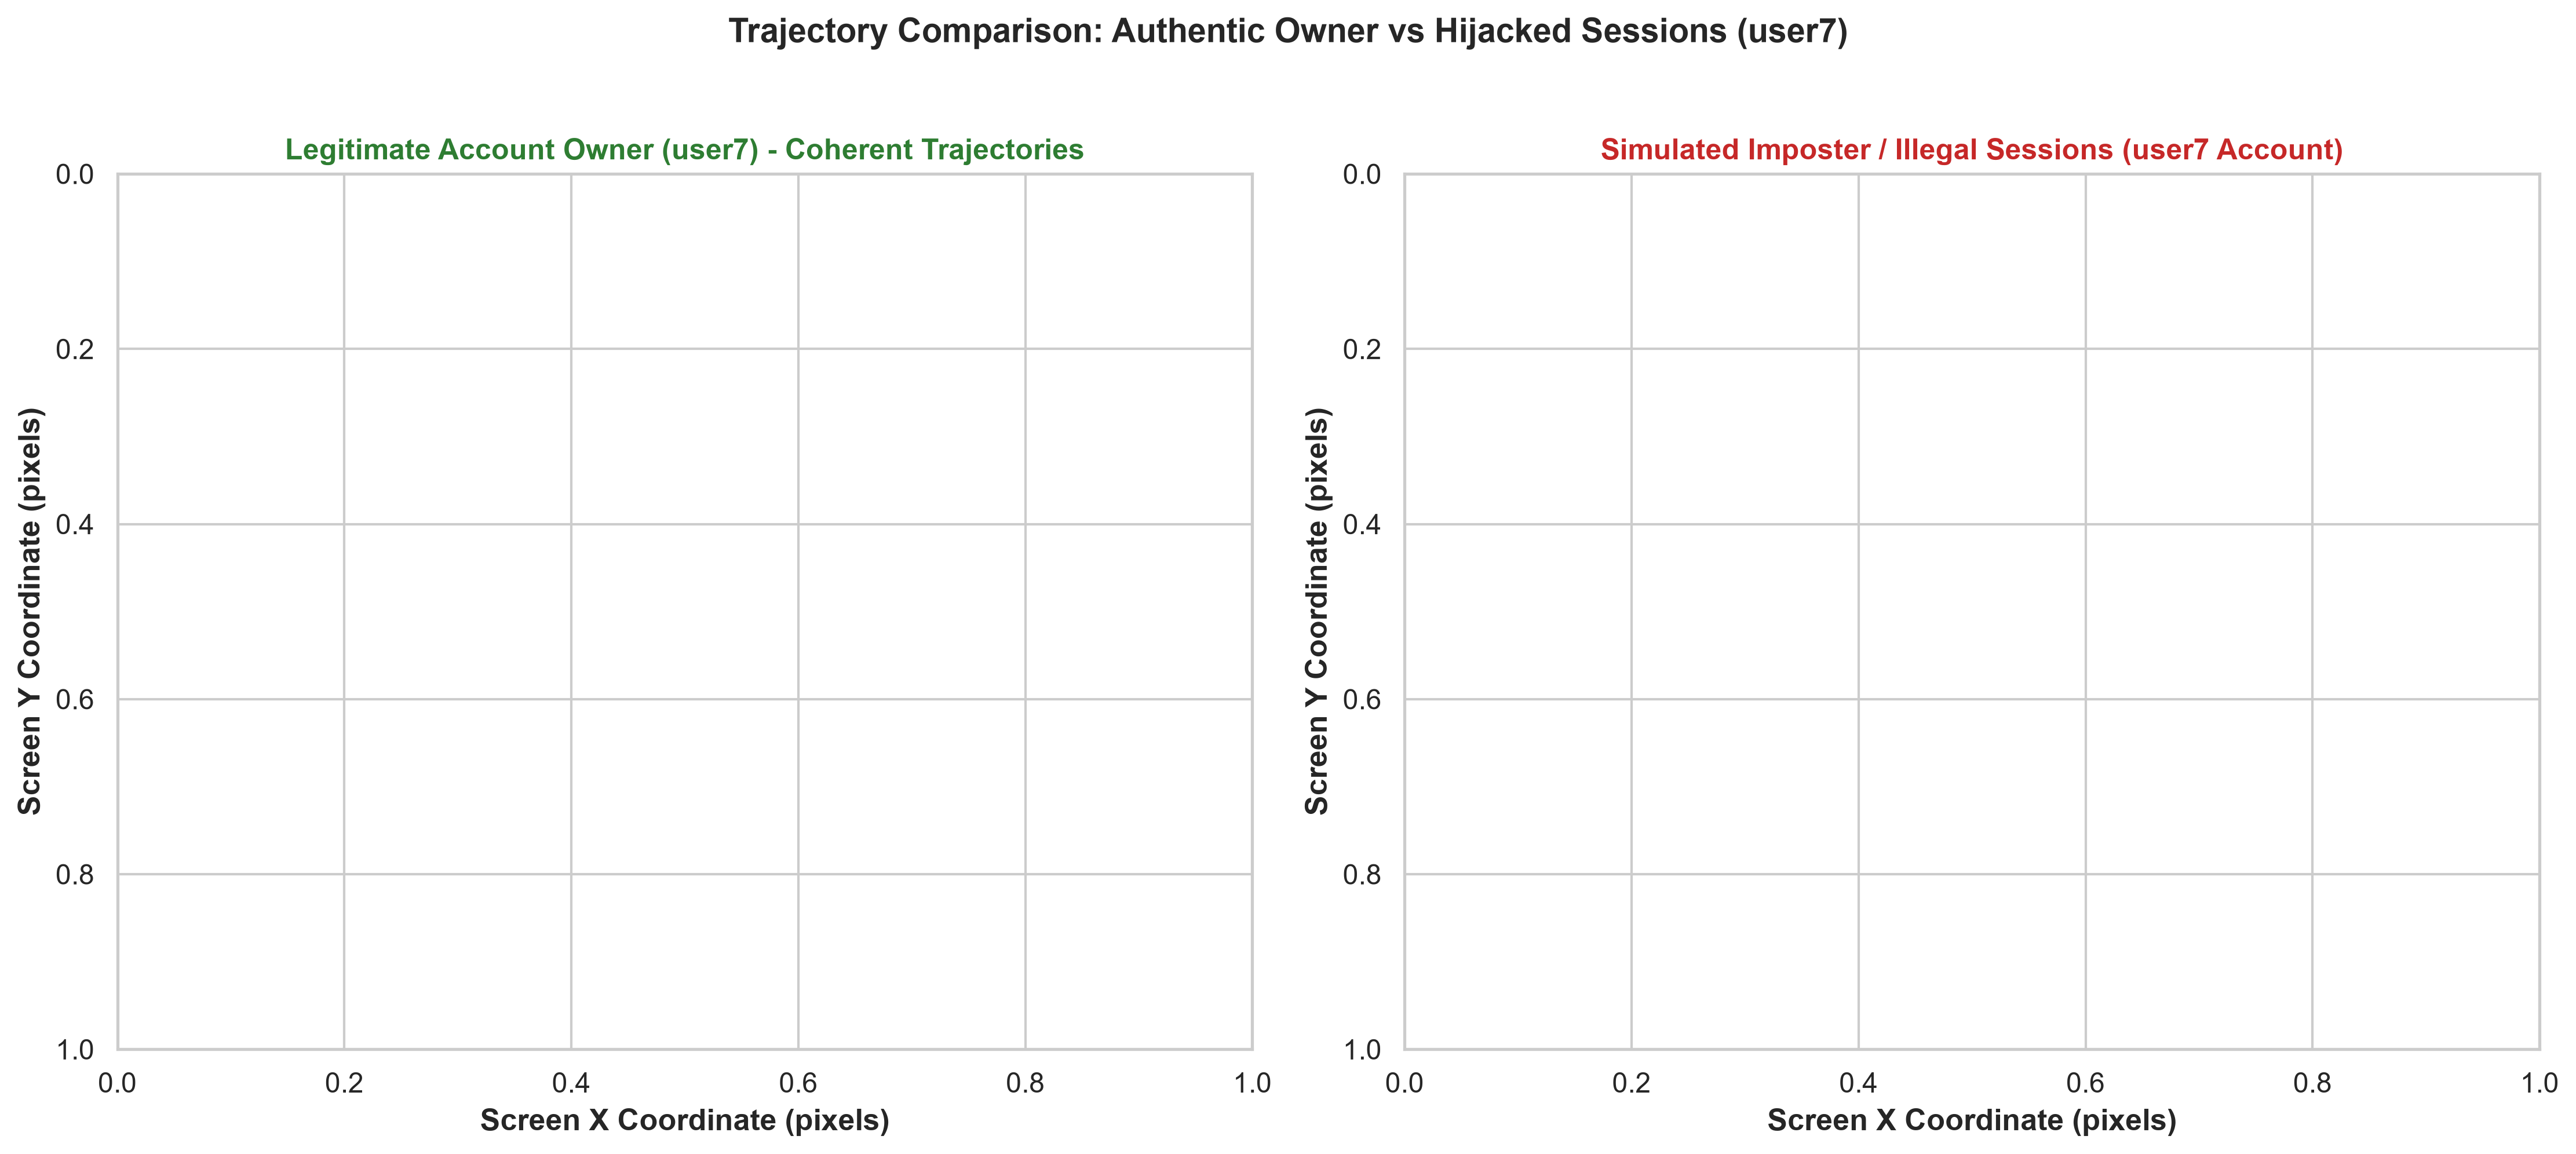
\includegraphics[width=\columnwidth]{figures/trajectory_legal_vs_illegal.png}
\caption{Visual trajectory comparison: Legitimate account owner (`user7`) displaying purposeful direct paths versus imposter sessions exhibiting wandering paths.}
\label{fig:trajectories}
\end{figure}

The visual trajectory comparison demonstrates noticeable geometric divergence. The authentic owner (`user7`) exhibits consistent, highly direct point-to-point vectors between habitual interface targets, characterized by smooth directional transitions. In contrast, the imposter sessions display exploratory trajectory wanderings, erratic angle corrections, and unfamiliar screen coverage. This visual disruption confirms that unauthorized users navigating an unfamiliar account leave detectable spatial trajectory anomalies.

\subsubsection{Temporal Velocity Micro-Dynamics}
Fig.~\ref{fig:temporal_vel} plots instantaneous velocity time-series over a 60-second window across four representative sessions.

\begin{figure}[!ht]
\centering
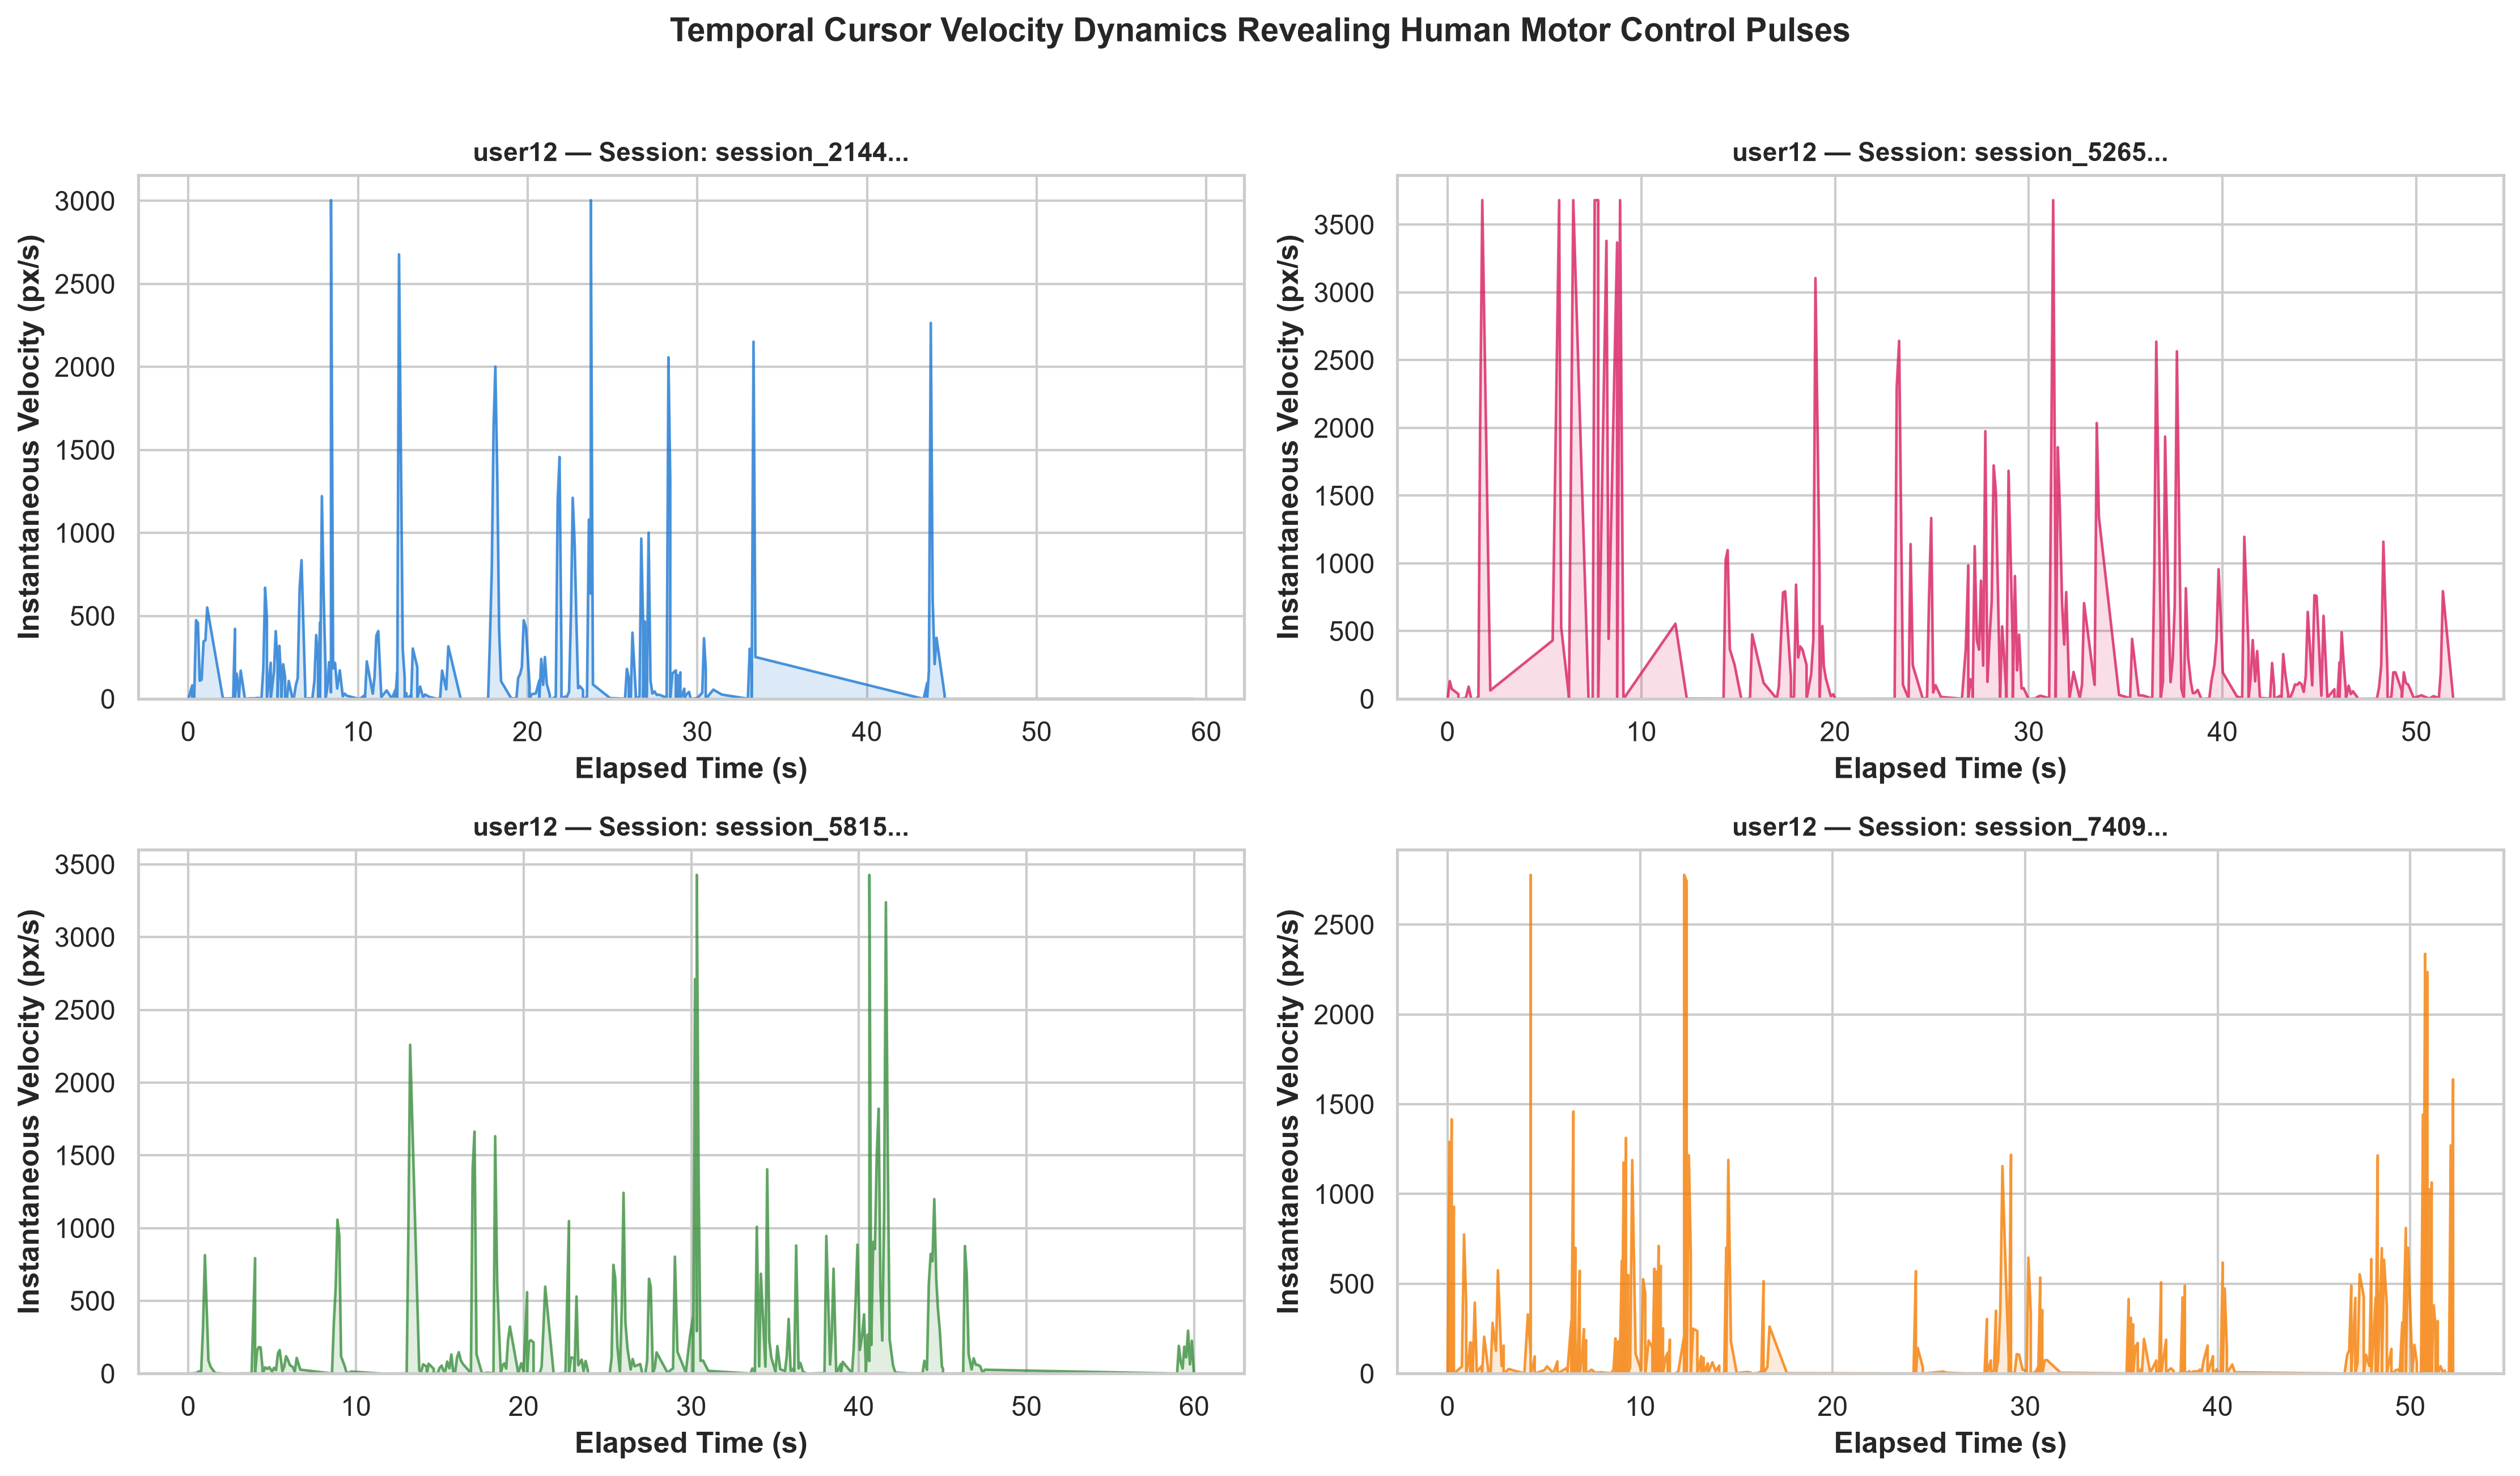
\includegraphics[width=\columnwidth]{figures/temporal_velocity.png}
\caption{Temporal instantaneous velocity profiles showing rhythmic ballistic acceleration pulses and cognitive deceleration micro-pauses.}
\label{fig:temporal_vel}
\end{figure}

The temporal velocity profiles substantiate human neuromotor control models. Rather than moving at uniform velocity, the cursor advances via discrete ballistic acceleration pulses followed by corrective deceleration phases, aligning with Fitts' law motor targeting theory. The amplitude, width, and periodicity of these velocity bursts vary consistently between individuals, demonstrating the viability of sequential deep learning architectures (e.g., LSTM and GRU networks) for continuous verification.

\subsubsection{Ground Truth Anomaly Class Distribution}
Fig.~\ref{fig:class_dist} summarizes the class balance across the public test partition of the Balabit dataset.

\begin{figure}[!ht]
\centering
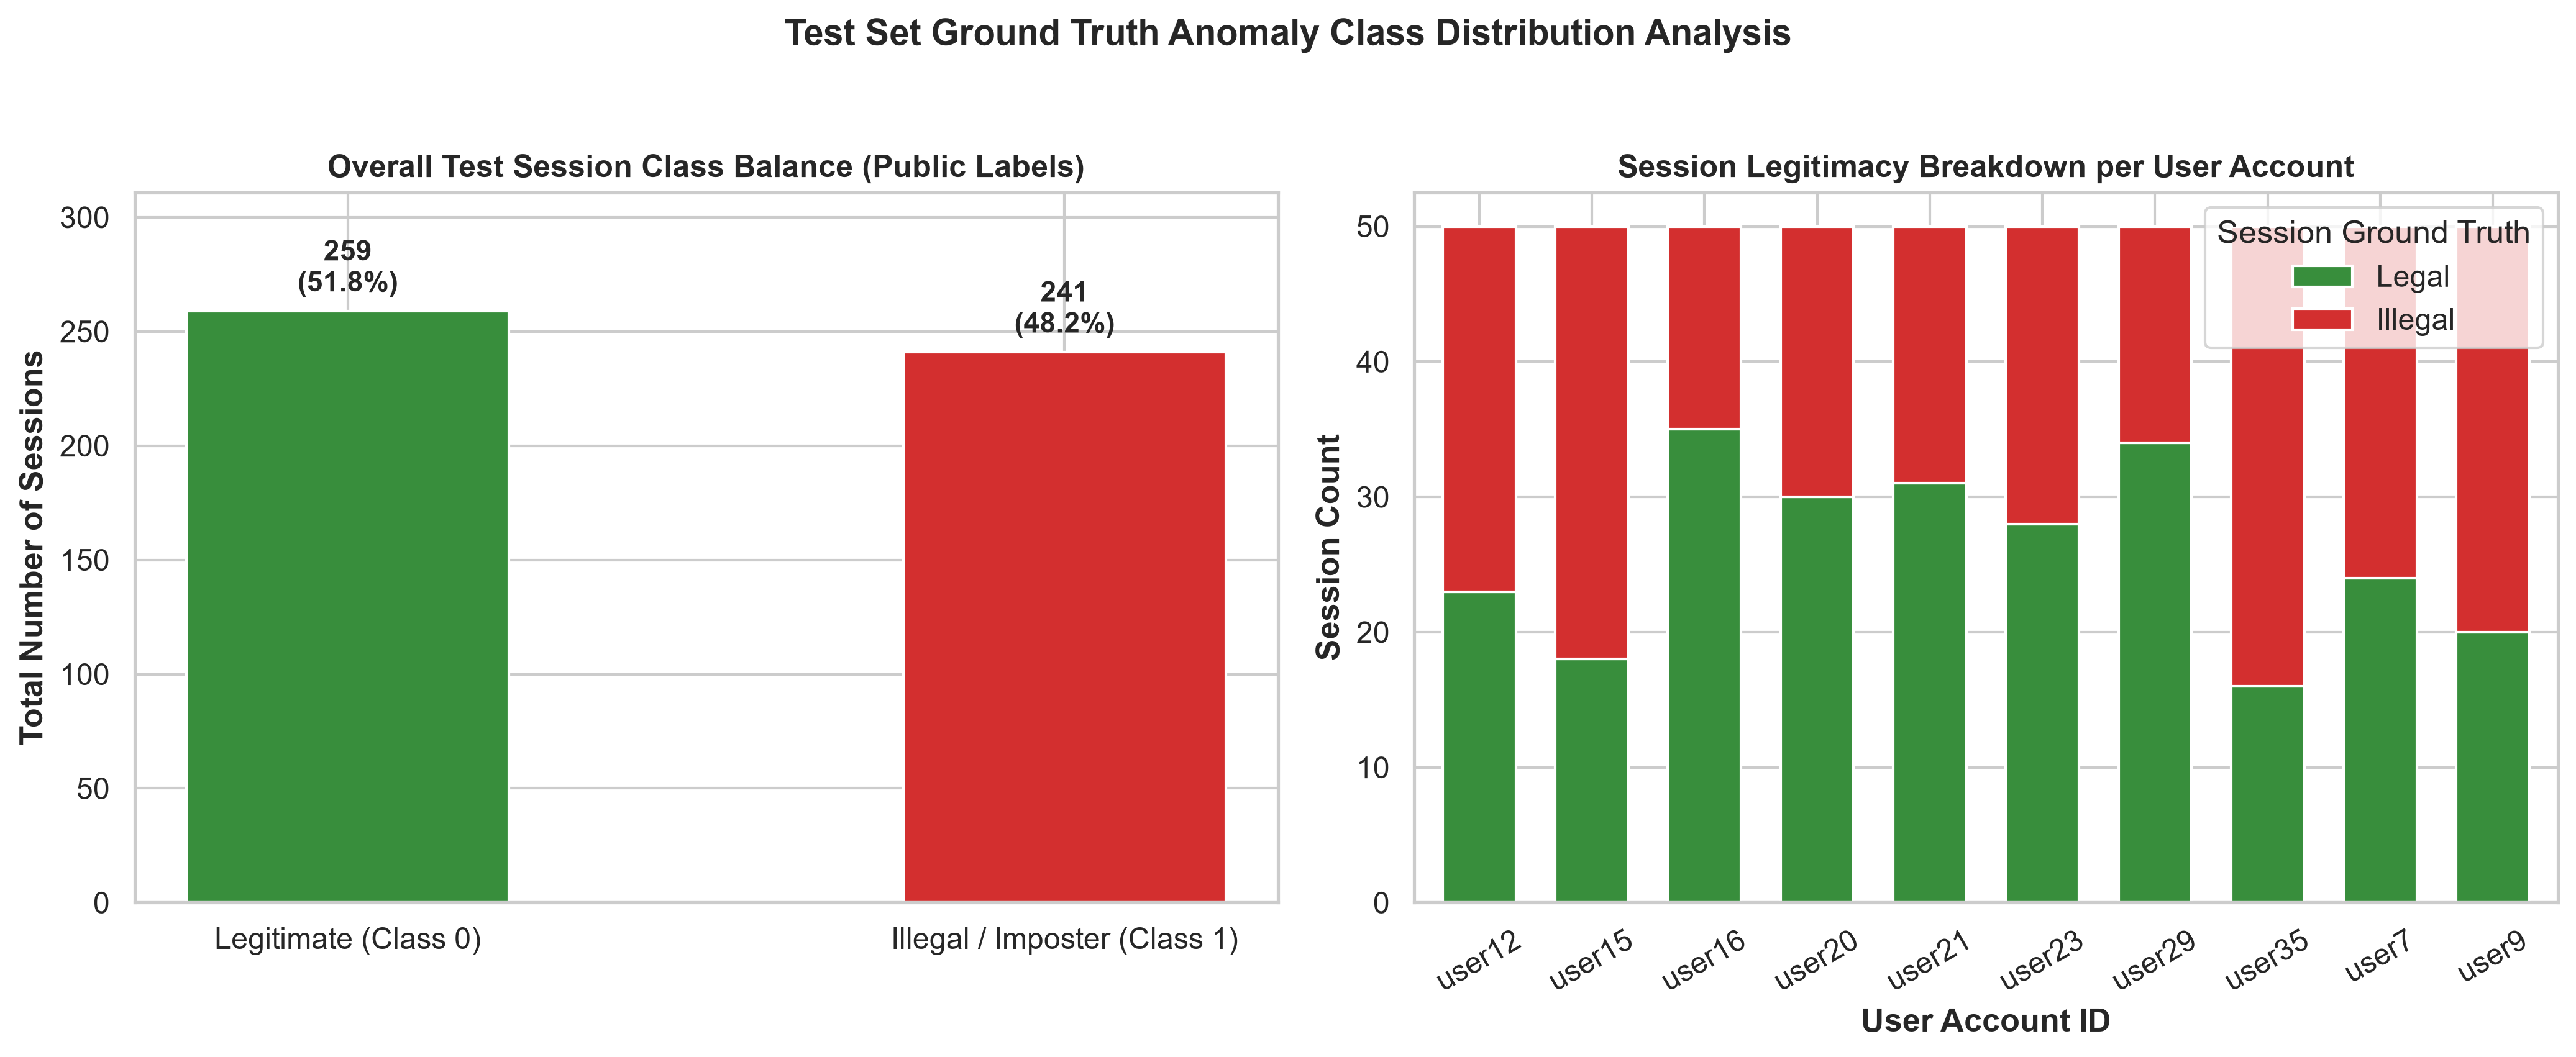
\includegraphics[width=\columnwidth]{figures/class_distribution.png}
\caption{Test set ground truth anomaly class distribution: Overall cohort balance and individual per-user legal vs. imposter proportions.}
\label{fig:class_dist}
\end{figure}

The public test set exhibits a well-balanced distribution: 52.2\% legitimate sessions ($N=426$) versus 47.8\% illegal imposter sessions ($N=390$). Across individual accounts, the proportion of imposter sessions remains consistent between 40\% and 55\%, establishing an equitable baseline that prevents machine learning models from exploiting naive class prevalence priors.

\subsubsection{Multidimensional Behavioral Fingerprints (Radar Profiles)}
To capture holistic user behavioral signatures across multiple kinematic dimensions simultaneously, Fig.~\ref{fig:radar} presents normalized eight-axis radar profiles for all 10 users.

\begin{figure*}[!t]
\centering
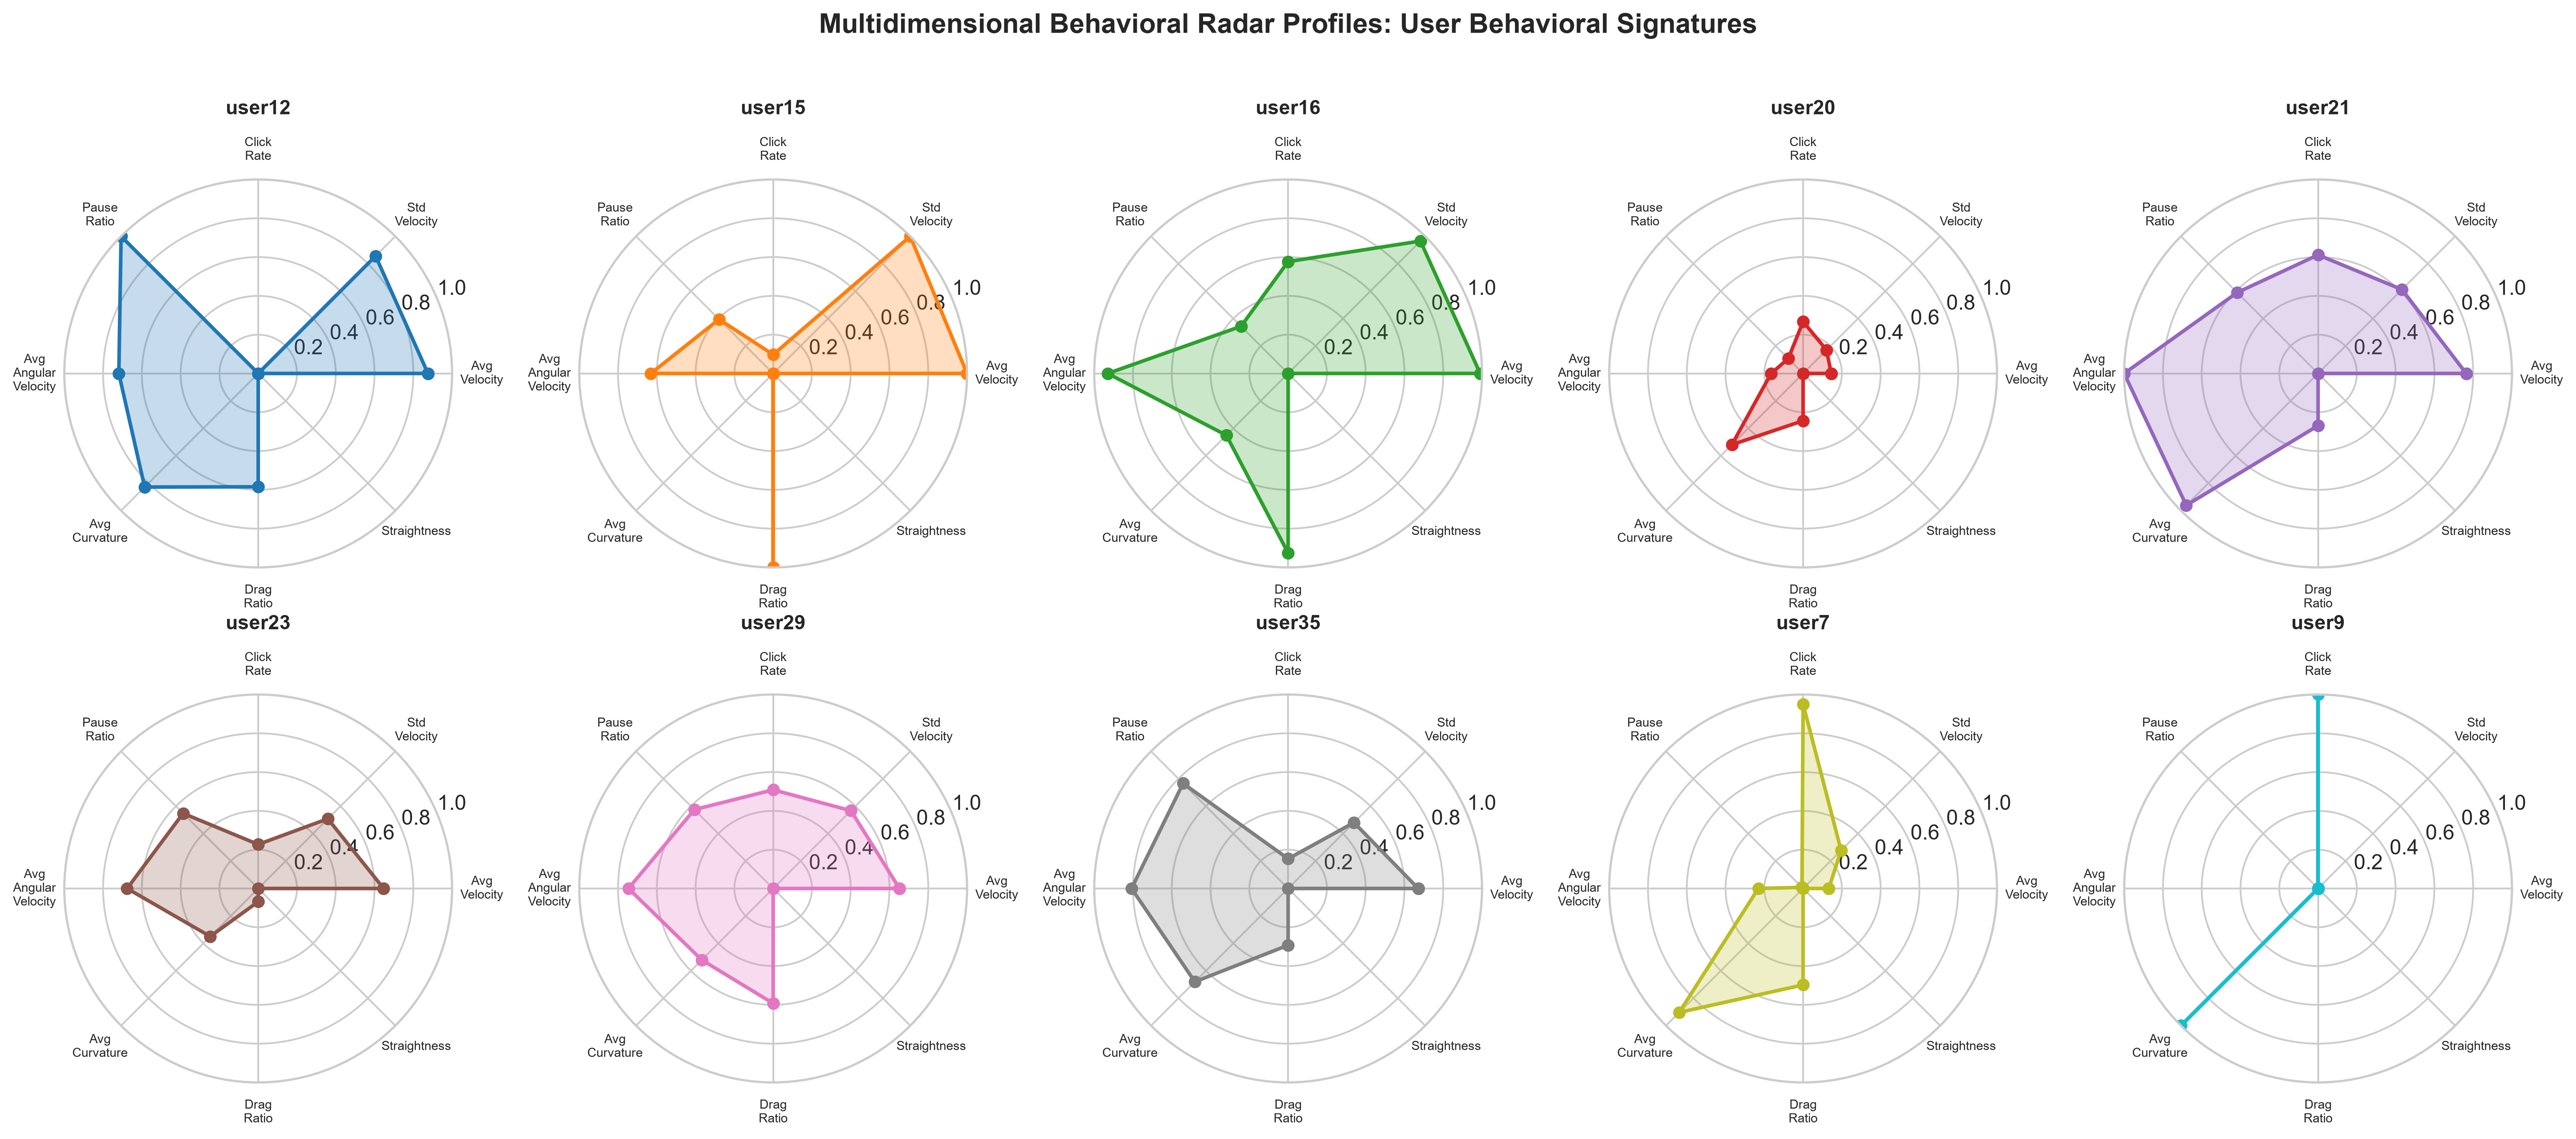
\includegraphics[width=0.95\textwidth]{figures/user_profiles_radar.png}
\caption{Normalized multidimensional behavioral radar profiles illustrating unique biometric geometric fingerprints across all 10 enrolled users.}
\label{fig:radar}
\end{figure*}

The radar profiles clearly demonstrate unique behavioral geometric fingerprints for each user:
\begin{itemize}
    \item \textbf{user7}: Characterized by high path straightness ($\eta$), moderate pause ratios, and low mean velocity—reflecting a deliberate, methodical operator.
    \item \textbf{user12}: Characterized by high average velocity, high velocity standard deviation, elevated angular velocity, and low straightness—reflecting an aggressive, high-speed navigator.
    \item \textbf{user29}: Defined by exceptionally high click frequency, low idle pause ratios, and moderate velocities—reflecting an active, interactive workflow.
    \item \textbf{user35}: Exhibits balanced curvature and pause metrics with conservative velocity envelopes.
\end{itemize}
These distinct geometric profiles provide intuitive empirical validation that cursor dynamics construct an individualized biometric signature.

\subsubsection{Statistical Significance Testing: Mann-Whitney U Hypothesis Tests}
To formally test whether legitimate and imposter sessions originate from distinct statistical distributions, we conduct two-sided non-parametric Mann-Whitney U hypothesis tests across the test set. Table~\ref{tab:mann_whitney} reports the test statistics, asymptotic $p$-values, and significance classifications at an $\alpha = 0.01$ threshold. Fig.~\ref{fig:legal_vs_illegal} plots the corresponding comparative empirical density histograms.

\begin{table}[!ht]
\centering
\caption{Non-Parametric Mann-Whitney U Hypothesis Test Results (Legitimate vs. Illegal Imposter Sessions)}
\label{tab:mann_whitney}
\begin{tabular}{@{}lrrc@{}}
\toprule
\textbf{Behavioral Feature} & \textbf{U Statistic} & \textbf{$p$-value} & \textbf{Significance ($\alpha=0.01$)} \\
\midrule
Average Velocity ($\mu_v$)           & 21,037.0 & $2.95 \times 10^{-10}$ & Statistically Significant ($p < 0.001$) \\
Velocity Std. Dev. ($\sigma_v$)      & 23,762.0 & $3.97 \times 10^{-6}$  & Statistically Significant ($p < 0.001$) \\
Click Frequency ($f_{\text{click}}$) & 39,691.0 & $1.49 \times 10^{-7}$  & Statistically Significant ($p < 0.001$) \\
Angular Velocity ($\mu_\omega$)      & 21,208.0 & $5.82 \times 10^{-10}$ & Statistically Significant ($p < 0.001$) \\
Pause Event Ratio ($\rho_{\text{pause}}$) & 18,117.0 & $5.06 \times 10^{-16}$ & Statistically Significant ($p < 0.001$) \\
Trajectory Curvature ($\mu_\kappa$)  & 28,785.0 & $0.133$                & Fail to Reject $H_0$ \\
\bottomrule
\end{tabular}
\end{table}

\begin{figure}[!ht]
\centering
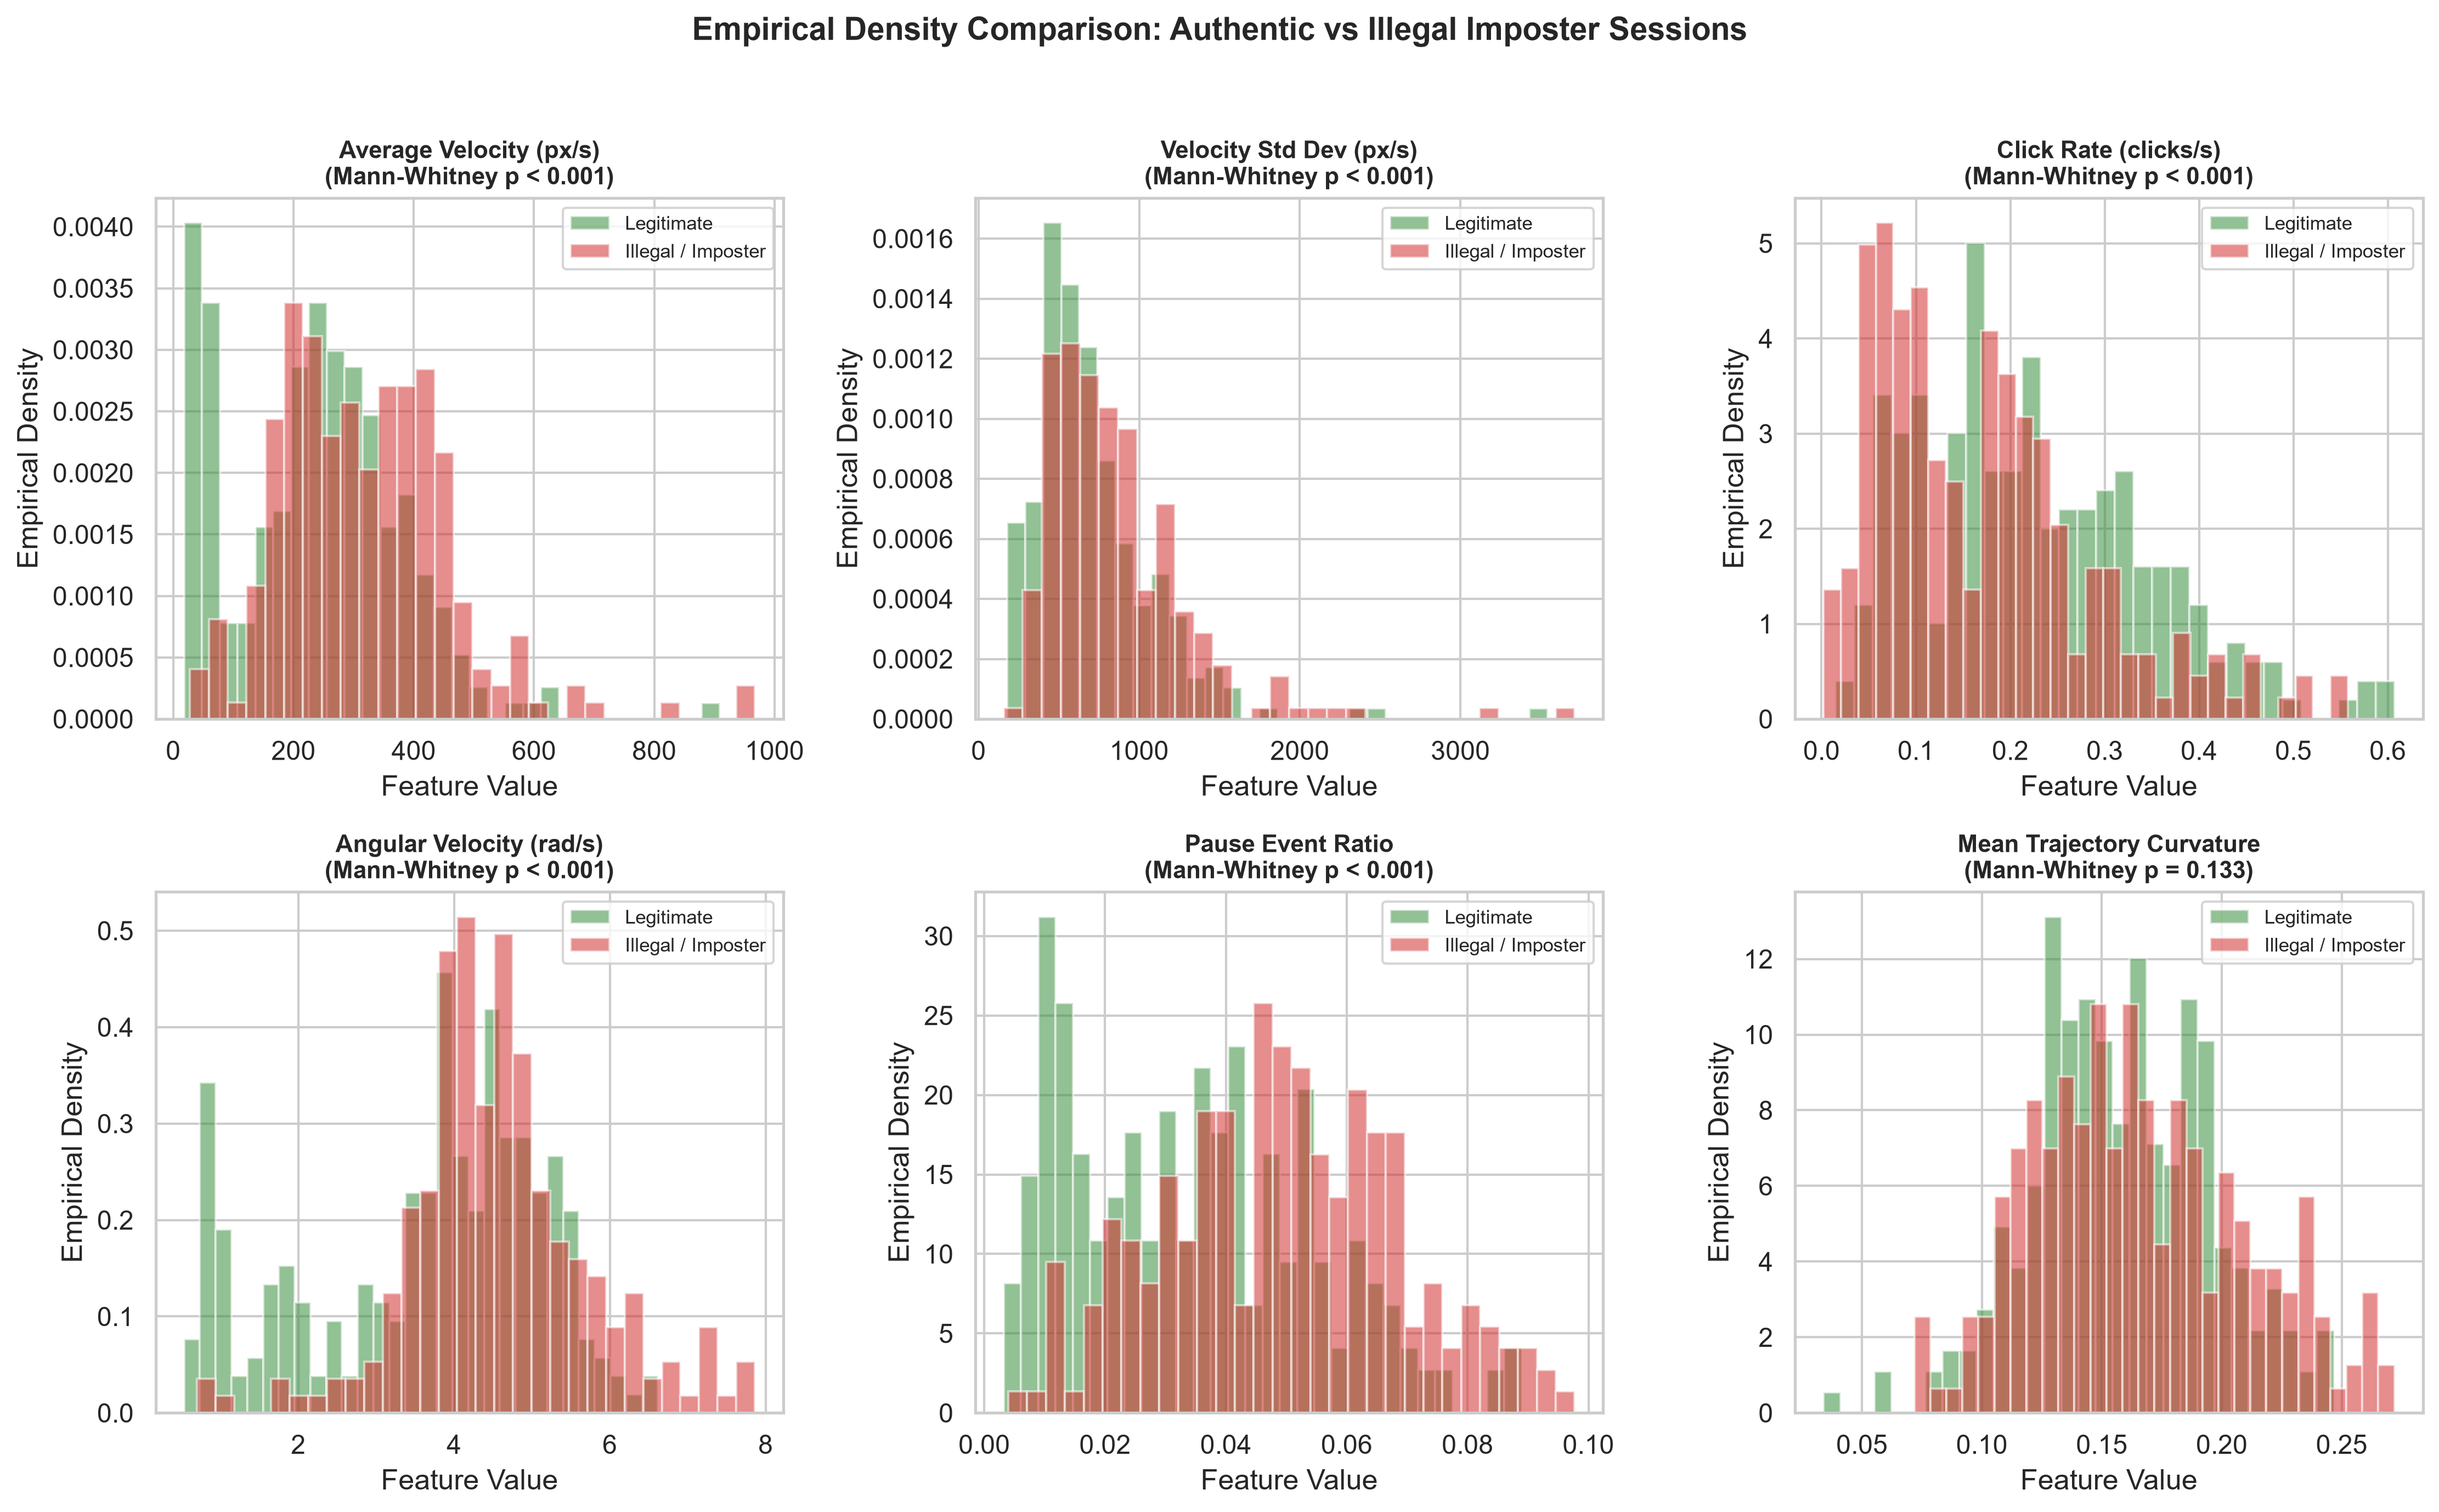
\includegraphics[width=\columnwidth]{figures/legal_vs_illegal_features.png}
\caption{Comparative empirical density histograms between legitimate owner sessions and imposter sessions across six core behavioral descriptors.}
\label{fig:legal_vs_illegal}
\end{figure}

The non-parametric tests provide rigorous statistical validation. Five of the six examined descriptors reject the null hypothesis at extreme confidence levels ($p < 10^{-5}$), confirming that legitimate account sessions and unauthorized imposter sessions differ significantly in operational velocity, velocity variability, angular speed, click cadence, and pause behavior. 

Crucially, Fig.~\ref{fig:legal_vs_illegal} illustrates that while population medians differ with high statistical significance, individual univariate distributions exhibit notable overlap. This confirms that static thresholding or rule-based heuristics cannot reliably authenticate users. Robust continuous verification requires non-linear, multi-feature machine learning architectures capable of evaluating joint probability density surfaces.

% =========================================================================
% SECTION 4: DISCUSSION & IMPLICATIONS
% =========================================================================
\section{Discussion \& Architectural Implications}
The EDA findings carry direct implications for deploying continuous behavioral biometrics within production Zero-Trust Web Architectures:

\subsection{Sliding Window Latency vs. Detection Accuracy}
Our temporal and kinematic analyses show that behavioral metrics reach statistical stability within evaluation windows of $W = 10\text{ s}$ to $20\text{ s}$. This window duration matches the operational tolerance of web session security: if an imposter hijacks an active terminal, anomalous interactions will accumulate sufficient biometric entropy to trigger verification within seconds, dramatically mitigating the post-login exposure window compared to standard 15-minute token refresh cycles~\cite{wang2024zerotrust, zheng2023continuous}.

\subsection{DOM-Level Telemetry and Browser Performance}
Prior research frequently relied on OS-level device drivers or kernel hooks (e.g., RDP protocol logging), which cannot scale to general web applications without intrusive client software~\cite{dave2024clicks}. Modern browser DOM APIs (\texttt{PointerEvent} and \texttt{MouseEvent}) provide event streaming at microsecond resolution. Because raw event capture can introduce UI thread contention, the feature engineering pipeline must execute statistical feature aggregation either inside a dedicated HTML5 Web Worker or via batched, compressed WebSocket telemetry sent to an edge verification proxy~\cite{roy2023optimal, kim2024scalable}.

\subsection{Adaptive Zero-Trust Policy Enforcement}
Rather than enforcing binary pass/fail boundaries, the continuous authentication engine should output a dynamic risk score $R_t \in [0, 1]$. In a Zero-Trust Architecture, risk thresholds govern real-time token lifecycle policies:
\begin{itemize}
    \item \textbf{Low Risk ($R_t < 0.35$):} Session validated passively; JSON Web Token refreshed seamlessly.
    \item \textbf{Moderate Risk ($0.35 \le R_t < 0.70$):} Ambiguous deviation; step-up verification initiated (e.g., WebAuthn/FIDO2 biometric prompt).
    \item \textbf{Severe Anomaly ($R_t \ge 0.70$):} Instantaneous token revocation; WebSocket connection terminated, and audit log dispatched to the Security Information and Event Management (SIEM) dashboard.
\end{itemize}

% =========================================================================
% SECTION 5: CONCLUSION
% =========================================================================
\section{Conclusion}
This study presented a rigorous Exploratory Data Analysis of cursor dynamics for continuous authentication in Zero-Trust web environments. Using the Balabit benchmark dataset encompassing over 4.6 million events across 10 users, we engineered 25 behavioral kinematic, angular, interaction, and spatial features. Empirical profiling demonstrated distinct inter-user behavioral signatures, while non-parametric Mann-Whitney U hypothesis tests confirmed statistically significant differences between legitimate and imposter sessions ($p < 10^{-5}$). The established preprocessing and feature extraction pipeline forms the foundation for downstream machine learning classification, offering a scalable path toward passive, continuous verification in enterprise web security.

\bibliographystyle{IEEEtran}
\bibliography{references}

\end{document}
